        %%******************************************%%
        %%                                          %%
        %%        Modello di tesi di laurea         %%
        %%            di Andrea Giraldin            %%
        %%                                          %%
        %%             2 novembre 2012              %%
        %%                                          %%
        %%******************************************%%


% I seguenti commenti speciali impostano:
% 1. 
% 2. PDFLaTeX come motore di composizione;
% 3. tesi.tex come documento principale;
% 4. il controllo ortografico italiano per l'editor.

% !TEX encoding = UTF-8
% !TEX TS-program = pdflatex
% !TEX root = tesi.tex
% !TEX spellcheck = it-IT

\documentclass[10pt,                    % corpo del font principale
               a4paper,                 % carta A4
               twoside,                 % impagina per fronte-retro
               openright,               % inizio capitoli a destra
               english,                 
               italian,                 
               ]{book}    

\usepackage[utf8]{inputenc}             % codifica di input; anche [latin1] va bene
                                        % NOTA BENE! va accordata con le preferenze dell'editor

%**************************************************************
% Importazione package
%************************************************************** 

%\usepackage{amsmath,amssymb,amsthm}    % matematica

\usepackage[english, italian]{babel}    % per scrivere in italiano e in inglese;
                                        % l'ultima lingua (l'italiano) risulta predefinita

\usepackage{bookmark}                   % segnalibri

\usepackage{caption}                    % didascalie

\usepackage{chngpage,calc}              % centra il frontespizio

\usepackage{csquotes}                   % gestisce automaticamente i caratteri (")

\usepackage{emptypage}                  % pagine vuote senza testatina e piede di pagina

\usepackage{epigraph}					% per epigrafi

\usepackage{eurosym}                    % simbolo dell'euro

\usepackage[T1]{fontenc}                % codifica dei font:
                                        % NOTA BENE! richiede una distribuzione *completa* di LaTeX

%\usepackage{indentfirst}               % rientra il primo paragrafo di ogni sezione

\usepackage{graphicx}                   % immagini

\usepackage{hyperref}                   % collegamenti ipertestuali



\usepackage[binding=5mm]{layaureo}      % margini ottimizzati per l'A4; rilegatura di 5 mm

\usepackage{listings}                   % codici

\usepackage{microtype}                  % microtipografia

\usepackage{mparhack,fixltx2e,relsize}  % finezze tipografiche

\usepackage{nameref}                    % visualizza nome dei riferimenti                                      

\usepackage[font=small]{quoting}        % citazioni

\usepackage{subfig}                     % sottofigure, sottotabelle

\usepackage[italian]{varioref}          % riferimenti completi della pagina

\usepackage[dvipsnames]{xcolor}         % colori

\usepackage{booktabs}                   % tabelle                                       
\usepackage{tabularx}                   % tabelle di larghezza prefissata                                    
\usepackage{longtable}                  % tabelle su più pagine                                        
\usepackage{ltxtable}                   % tabelle su più pagine e adattabili in larghezza

\usepackage[toc, acronym]{glossaries}   % glossario
                                        % per includerlo nel documento bisogna:
                                        % 1. compilare una prima volta tesi.tex;
                                        % 2. eseguire: makeindex -s tesi.ist -t tesi.glg -o tesi.gls tesi.glo
                                        % 3. eseguire: makeindex -s tesi.ist -t tesi.alg -o tesi.acr tesi.acn
                                        % 4. compilare due volte tesi.tex.

\usepackage[backend=biber,style=verbose-ibid,hyperref,backref]{biblatex}
                                        % eccellente pacchetto per la bibliografia; 
                                        % produce uno stile di citazione autore-anno; 
                                        % lo stile "numeric-comp" produce riferimenti numerici
                                        % per includerlo nel documento bisogna:
                                        % 1. compilare una prima volta tesi.tex;
                                        % 2. eseguire: biber tesi
                                        % 3. compilare ancora tesi.tex.

%**************************************************************
% file contenente le impostazioni della tesi
%**************************************************************

%**************************************************************
% Frontespizio
%**************************************************************
\newcommand{\myName}{Giacomo Manzoli\xspace}                                    % autore
\newcommand{\myTitle}{Sviluppo di applicazioni native per iOS in JavaScript}                    
\newcommand{\myDegree}{Tesi di laurea triennale}                % tipo di tesi
\newcommand{\myUni}{Università degli Studi di Padova}           % università
\newcommand{\myFaculty}{Corso di Laurea in Informatica}         % facoltà
\newcommand{\myDepartment}{Dipartimento di Matematica}          % dipartimento
\newcommand{\myProf}{Claudio Enrico Palazzi\xspace}                                % relatore
\newcommand{\myLocation}{Padova\xspace}                                % dove
\newcommand{\myAA}{2014-2015\xspace}                                   % anno accademico
\newcommand{\myTime}{Ottobre 2015\xspace}                                  % quando

\newcommand{\myCompany}{WARDA S.r.l.\xspace}

\newcommand{\glossario}[1]{\textit{#1\ped{\ped{G}}}}            % per il glossario



%**************************************************************
% Impostazioni di impaginazione
% see: http://wwwcdf.pd.infn.it/AppuntiLinux/a2547.htm
%**************************************************************

\setlength{\parindent}{14pt}   % larghezza rientro della prima riga
\setlength{\parskip}{0pt}   % distanza tra i paragrafi


%**************************************************************
% Impostazioni di biblatex
%**************************************************************
\bibliography{bibliografia} % database di biblatex 

\defbibheading{bibliography}
{
    %\cleardoublepage
    %\clearpage
    \phantomsection 
    %\addcontentsline{toc}{chapter}{\bibname}
    \addcontentsline{toc}{chapter}{Riferimenti}
    \chapter*{\bibname\markboth{\bibname}{\bibname}}
}

\setlength\bibitemsep{1.5\itemsep} % spazio tra entry

\DeclareBibliographyCategory{web}


\defbibheading{web}{\section*{Siti Web di riferimento}}


%**************************************************************
% Impostazioni di caption
%**************************************************************
\captionsetup{
%    tableposition=top,
    figureposition=bottom,
    font=small,
    format=hang,
    labelfont=bf
}

%**************************************************************
% Impostazioni di glossaries
%**************************************************************

%**************************************************************
% Acronimi
%**************************************************************
\renewcommand{\acronymname}{Acronimi e abbreviazioni}

\newacronym[description={\glslink{apig}{Application Program Interface}}]
    {api}{API}{Application Program Interface}
    
\newacronym[description={\glslink{html}{HyperText Markup Language}}]
    {html}{HTML}{HyperText Markup Language}

\newacronym[description={\glslink{rest}{Representational State Transfer}}]
    {rest}{REST}{Representational State Transfer}   

\newacronym[description={\glslink{virtualmachine}{Virtual Machine}}]
    {vm}{VM}{Virtual Machine}   


%**************************************************************
% Glossario
%**************************************************************
\renewcommand{\glossaryname}{Glossario}

\newglossaryentry{Cordova}
{
    name=\glslink{Cordova}{Cordova},
    text=Cordova,
    sort=Cordova,
    description={Apache Cordova è un framework open source per la realizzazione di applicazioni ibride che offre delle API che permettono di accedere via JavaScript ad alcune funzionalità native del dispositivo, come l'accelerometro o la fotocamera}
}

\newglossaryentry{PhoneGap}
{
    name=\glslink{PhoneGap}{PhoneGap},
    text=PhoneGap,
    sort=PhoneGap,
    description={Framework che permette la realizzazione di applicazioni mobile ibride e multi piattaforma utilizzando HTML, CSS e JavaScript. Questo framework è stato pubblicato da Adobe e utilizza Apache Cordova per   interagire con le funzionalità native offerte dai vari sistemi operativi}
}


\newglossaryentry{virtual machine}
{
    name=\glslink{virtual machine}{Virtual machine},
    text=virtual machine,
    sort=virtual machine,
    description={Software che simula delle risorse hardware e che utilizza queste risorse per eseguire determinate applicazione, in modo che queste possano utilizzare le risorse simulate. Le virtual machine hanno vari utilizzi, in questo caso vengono utilizzate per interpretare il codice JavaScript}
}

\newglossaryentry{DOM}
{
    name=\glslink{DOM}{DOM},
    text=DOM,
    sort=DOM,
    description={Il DOM o \textit{Document Object Model} è lo standard del W3C per la rappresentazione ad oggetti di documenti strutturati, come le pagine HTML}
}

\newglossaryentry{WebView}
{
    name=\glslink{WebView}{WebView},
    text=WebView,
    sort=WebView,
    description={Componente grafico offerto dalle API native, sia di iOS, sia di Android, che permette la visualizzazione di pagine HTML}
}

\newglossaryentry{rendering}
{
    name=\glslink{rendering}{Rendering},
    text=rendering,
    sort=rendering,
    description={Termine inglese che indica l'insieme di attività da svolgere per la rappresentazione grafica di un elemento, nel caso specifico dell'interfaccia grafica di un'applicazione}
}

\newglossaryentry{npm}
{
    name=\glslink{npm}{npm},
    text=npm,
    sort=npm,
    description={Acronimo di Node Package Manager, è un sistema di gestione delle dipendenze per le applicazioni JavaScript che permette di installare librerie di terze parti mediante un'interfaccia a riga di comando}
}

\newglossaryentry{riflessione}
{
    name=\glslink{riflessione}{Riflessione},
    text=riflessione,
    sort=riflessione,
    description={In informatica, è la capacità di un programma di analizzare, durante la sua esecuzione, le classi che lo compongono, ricavando così informazioni sulla struttura del proprio codice sorgente}
}
    
\newglossaryentry{gesture}
{
    name=\glslink{gesture}{Gesture},
    text=gesture,
    sort=gesture,
    description={Combinazione di movimenti dell'utente effettuati con le dita su un dispositivo touch-screen, che vengono riconosciuti da un'applicazione}
}

\newglossaryentry{tap}
{
    name=\glslink{tap}{Tap},
    text=tap,
    sort=tap,
    description={Gesture che consiste in un singolo tocco dello schermo da parte dell'utente, è l'equivalente di un click del mouse}
}

\newglossaryentry{pan}
{
    name=\glslink{pan}{Pan},
    text=pan,
    sort=pan,
    description={Gesture che consiste in un tocco prolungato dello schermo da parte dell'utente. Durante l'esecuzione della gesture, l'utente può trascinare il punto di contatto in un modo simile al \textit{drag'n'drop} effettuato con il mouse}
}

\newglossaryentry{swipe}
{
    name=\glslink{swipe}{Swipe},
    text=swipe,
    sort=swipe,
    description={\`E un particolare tipo di pan, effettuato in modo rapito e in una singola direzione, tipicamente da destra verso sinistra o viceversa}
}

\newglossaryentry{pinch-to-zoom}
{
    name=\glslink{pinch-to-zoom}{Pinch-to-zoom},
    text=pinch-to-zoom,
    sort=pinch-to-zoom,
    description={\`E la gesture che viene utilizzata per eseguire lo zoom su un elemento dell'interfaccia grafica, tipicamente un'immagine o una pagina web. Questa gesture consiste nel toccare lo schermo con due dita e allontanarle o avvicinarle tra loro, senza mai staccarle dallo schermo. Nel caso le due dita vengano allontanate viene eseguito uno zoom del contenuto mentre nel caso contrario viene rimpicciolito}
}

\newglossaryentry{singleton}
{
    name=\glslink{singleton}{Singleton},
    text=singleton,
    sort=singleton,
    description={Il singleton è un design pattern individuato dalla \textit{Gang of Four} che ha lo scopo di garantire che venga creata una sola istanza di una determinata classe, e di fornire un punto di accesso globale a tale istanza.
     Nel progetto questo pattern viene implementato sfruttando i moduli CommonJS, creando l'istanza di un oggetto, per poi esportarla come modulo. In questo modo l'oggetto viene creato solo una volta e risulta accessibile a tutta l'applicazione in quanto è un normale modulo CommonJS}
}

\newglossaryentry{proxy}
{
    name=\glslink{proxy}{Proxy},
    text=proxy,
    sort=proxy,
    description={Il proxy è un design pattern individuato dalla \textit{Gang of Four} che prevede l'utilizzo di un classe o oggetto come interfaccia per qualche altro oggetto. Un esempio di utilizzo di questo pattern è dato da Java RMI, che mediante l'utilizzo di oggetti remoti, nasconde la complessità legata al fatto che l'oggetto vero e proprio sul quale viene invocato il metodo si trova su un computer diverso. Nel caso di NativeScript, viene utilizzato un oggetto JavaScript come interfaccia di un oggetto nativo (che può essere sia un oggetto Obj-C, sia Java) in modo che l'oggetto nativo possa essere utilizzato via JavaScript}
}


\newglossaryentry{popover}
{
    name=\glslink{popover}{Popover},
    text=popover,
    sort=popover,
    description={Un popover è un componente delle interfacce grafiche simile ad un pop-up, che compare quanto l'utente seleziona un elemento. A differenza di un pop-up che compare al centro dello schermo, un popover compare vicino al pulsante che l'ha reso visibile ed è collegato ad esse mediante una freccia}
}

\newglossaryentry{API}
{
    name=\glslink{API}{API},
    text=API,
    sort=API,
    description={Indica un'insieme di procedure rese disponibili al programmatore allo scopo di ottenere un'astrazione della complessità della piattaforma sottostante, che può essere sia hardware che software}
}

\newglossaryentry{V8}
{
    name=\glslink{V8}{V8},
    text=V8,
    sort=V8,
    description={V8 è un motore JavaScript open source sviluppato da Google, attualmente incluso in Google Chrome}
}

\newglossaryentry{JavaScriptCore}
{
    name=\glslink{JavaScriptCore}{JavaScriptCore},
    text=JavaScriptCore,
    sort=JavaScriptCore,
    description={JavaScriptCore è un motore JavaScript open source sviluppato da Apple, attualmente incluso in Safari e Safari Mobile}
}

\newglossaryentry{REST}
{
    name=\glslink{REST}{REST},
    text=REST,
    sort=REST,
    description={Riferisce ad un insieme di principi di architetture di rete, i quali delineano come le risorse sono definite e indirizzate. Il termine è spesso usato nel senso di descrivere ogni semplice interfaccia che trasmette dati su HTTP}
}

\newglossaryentry{SDK}
{
name=\glslink{SDK}{SDK},
text=SDK,
sort=SDK,
description={Acronimo di \textit{Software Development Kit}, insieme di strumenti per lo sviluppo e la documentazione di software}
}

\newglossaryentry{Obj-C}
{
    name=\glslink{Obj-C}{Obj-C},
    text=Obj-C,
    sort=Obj-C,
    description={Abbreviazione di Objective-C, un linguaggio di programmazione orientato agli oggetti derivato dal C. Questo linguaggio è stato scelto da Apple come strumento di sviluppo per le applicazione iOS e Mac OS X}
}

\newglossaryentry{MVC}
{
    name=\glslink{MVC}{MVC},
    text=MVC,
    sort=MVC,
    description={Pattern architetturale che prevede la separazione tra la logica di gestione dei dati e come questi dati vengono presentati. Il pattern prevede la divisione dell'architettura in tre parti: \textbf{Model}: si occupa della gestione dei dati; \textbf{View}: si occupa di visualizzare i dati presenti nel model; \textbf{Controller}: si occupa di aggiornare il model in base alle operazioni che l'utente compie sulla view}
}

\newglossaryentry{FPS}
{
name=\glslink{FPS}{FPS},
text=FPS,
sort=FPS,
description={\textit{fotogrammi per secondo}, è un unità di misura utilizzata per indicare la frequenza con la quale vengono generati dei fotogrammi}
}
 % database di termini
\makeglossaries


%**************************************************************
% Impostazioni di graphicx
%**************************************************************
\graphicspath{{immagini/}} % cartella dove sono riposte le immagini


%**************************************************************
% Impostazioni di hyperref
%**************************************************************
\hypersetup{
    %hyperfootnotes=false,
    %pdfpagelabels,
    %draft,	% = elimina tutti i link (utile per stampe in bianco e nero)
    colorlinks=true,
    linktocpage=true,
    pdfstartpage=1,
    pdfstartview=FitV,
    % decommenta la riga seguente per avere link in nero (per esempio per la stampa in bianco e nero)
    %colorlinks=false, linktocpage=false, pdfborder={0 0 0}, pdfstartpage=1, pdfstartview=FitV,
    breaklinks=true,
    pdfpagemode=UseNone,
    pageanchor=true,
    pdfpagemode=UseOutlines,
    plainpages=false,
    bookmarksnumbered,
    bookmarksopen=true,
    bookmarksopenlevel=1,
    hypertexnames=true,
    pdfhighlight=/O,
    %nesting=true,
    %frenchlinks,
    urlcolor=webbrown,
    linkcolor=RoyalBlue,
    citecolor=webgreen,
    %pagecolor=RoyalBlue,
    %urlcolor=Black, linkcolor=Black, citecolor=Black, %pagecolor=Black,
    pdftitle={\myTitle},
    pdfauthor={\textcopyright\ \myName, \myUni, \myFaculty},
    pdfsubject={},
    pdfkeywords={},
    pdfcreator={pdfLaTeX},
    pdfproducer={LaTeX}
}

%**************************************************************
% Impostazioni di itemize
%**************************************************************
%\renewcommand{\labelitemi}{$\ast$}

\renewcommand{\labelitemi}{$\bullet$}
%\renewcommand{\labelitemii}{$\cdot$}
%\renewcommand{\labelitemiii}{$\diamond$}
%\renewcommand{\labelitemiv}{$\ast$}


%**************************************************************
% Impostazioni di listings
%**************************************************************
\definecolor{codegreen}{rgb}{0,0.6,0}
\definecolor{codegray}{rgb}{0.5,0.5,0.5}
\definecolor{backcolor}{rgb}{0.98,0.98,0.98}

\renewcommand{\lstlistingname}{codice}% Listing -> codice
\renewcommand{\lstlistlistingname}{Frammenti di codice}% List of Listings -> Frammenti di codice

\lstdefinestyle{mystyle}{
    backgroundcolor=\color{backcolor},   
    commentstyle=\color{Peach}\ttfamily,
    keywordstyle=\color{RoyalBlue},
    numberstyle=\tiny\color{codegray},
    stringstyle=\color{SeaGreen}\ttfamily,
    basicstyle=\footnotesize\ttfamily,
    breakatwhitespace=false,         
    breaklines=true,                 
    captionpos=b,                    
    keepspaces=true,                 
    numbers=left,                    
    numbersep=5pt,                  
    showspaces=false,                
    showstringspaces=false,
    showtabs=false,                  
    tabsize=2,
    frame=trbl, % draw a frame at the top, right, left and bottom of the listing
	frameround=ftff, % angolo in basso a destro curvo
	framesep=4pt, % quarter circle size of the round corners,
}

 
\lstset{style=mystyle}

\lstdefinelanguage{JavaScript}
{
  % list of keywords
  morekeywords={ true, false, catch, function, break,	new, class, extends, var, require, switch, return, import, if, while, for, this, View, Text, StyleSheet},
  sensitive=false, % keywords are not case-sensitive
  morecomment=[l]{//}, % l is for line comment
  morecomment=[s]{/*}{*/}, % s is for start and end delimiter
  morestring=[b]' % defines that strings are enclosed in double quotes
}


%**************************************************************
% Impostazioni di xcolor
%**************************************************************
\definecolor{webgreen}{rgb}{0,.5,0}
\definecolor{webbrown}{rgb}{.6,0,0}


%**************************************************************
% Altro
%**************************************************************

\newcommand{\omissis}{[\dots\negthinspace]} % produce [...]

% eccezioni all'algoritmo di sillabazione
\hyphenation
{
    ma-cro-istru-zio-ne
    gi-ral-din
}

\newcommand{\sectionname}{Sezione}
\addto\captionsitalian{\renewcommand{\figurename}{Figura}
                       \renewcommand{\tablename}{Tabella}}

\newcommand{\glsfirstoccur}{\ap{{[g]}}}

\newcommand{\intro}[1]{\emph{\textsf{#1}}}

%**************************************************************
% Environment per ``TODO''
%**************************************************************

\newcommandx{\unsure}[2][1=]{\todo[linecolor=red,backgroundcolor=red!25,bordercolor=red,#1]{#2}}
\newcommandx{\change}[2][1=]{\todo[linecolor=blue,backgroundcolor=blue!25,bordercolor=blue,#1]{#2}}
\newcommandx{\info}[2][1=]{\todo[linecolor=OliveGreen,backgroundcolor=OliveGreen!25,bordercolor=OliveGreen,#1]{#2}}
\newcommandx{\improvement}[2][1=]{\todo[linecolor=Plum,backgroundcolor=Plum!25,bordercolor=Plum,#1]{#2}}
\newcommandx{\thiswillnotshow}[2][1=]{\todo[disable,#1]{#2}}                     % file con le impostazioni personali

\begin{document}
%**************************************************************
% Materiale iniziale
%**************************************************************
\frontmatter
% !TEX encoding = UTF-8
% !TEX TS-program = pdflatex
% !TEX root = ../tesi.tex
% !TEX spellcheck = it-IT

%**************************************************************
% Frontespizio 
%**************************************************************
\begin{titlepage}

\begin{center}

\begin{LARGE}
\textbf{\myUni}\\
\end{LARGE}

\vspace{10pt}

\begin{Large}
\textsc{\myDepartment}\\
\end{Large}

\vspace{10pt}

\begin{large}
\textsc{\myFaculty}\\
\end{large}

\vspace{30pt}
\begin{figure}[htbp]
\begin{center}

\includegraphics[height=6cm]{logo-unipd}
\end{center}
\end{figure}
\vspace{10pt} 

\begin{LARGE}
\begin{center}
\textbf{\myTitle}\\
\end{center}
\end{LARGE}

\vspace{10pt} 

\begin{large}
\textsl{\myDegree}\\
\end{large}

\vspace{40pt} 

\begin{large}
\begin{flushleft}
\textit{Relatore}\\ 
\vspace{5pt} 
Prof. \myProf
\end{flushleft}

\vspace{0pt} 

\begin{flushright}
\textit{Laureando}\\ 
\vspace{5pt} 
\myName
\end{flushright}
\end{large}

\vspace{40pt}

\line(1, 0){338} \\
\begin{normalsize}
\textsc{Anno Accademico \myAA}
\end{normalsize}

\end{center}
\end{titlepage} 
% !TEX encoding = UTF-8
% !TEX TS-program = pdflatex
% !TEX root = ../tesi.tex
% !TEX spellcheck = it-IT

%**************************************************************
% Colophon
%**************************************************************
\clearpage
\phantomsection
\thispagestyle{empty}

% !TEX encoding = UTF-8
% !TEX TS-program = pdflatex
% !TEX root = ../tesi.tex
% !TEX spellcheck = it-IT

%**************************************************************
% Sommario
%**************************************************************
\cleardoublepage
\phantomsection
\pdfbookmark{Sommario}{Sommario}
\begingroup
\let\clearpage\relax
\let\cleardoublepage\relax
\let\cleardoublepage\relax

\chapter*{Sommario}

Il presente documento descrive il lavoro svolto durante il periodo di stage, della durata di circa trecento ore, dal laureando \myName presso l'azienda \myCompany.
L'obiettivo di tale attività di stage è l'analisi dei vari framework disponibili per lo sviluppo di applicazioni native utilizzando il linguaggio JavaScript, al fine di creare un'applicazione nativa per iOS simili alla gallery sviluppata dall'azienda.
%\vfill
%
%\selectlanguage{english}
%\pdfbookmark{Abstract}{Abstract}
%\chapter*{Abstract}
%
%\selectlanguage{italian}

\endgroup			

\vfill


% !TEX encoding = UTF-8
% !TEX TS-program = pdflatex
% !TEX root = ../tesi.tex
% !TEX spellcheck = it-IT

%**************************************************************
% Ringraziamenti
%**************************************************************
\cleardoublepage
\phantomsection
\pdfbookmark{Ringraziamenti}{ringraziamenti}

\begin{flushright}{
 \slshape    
 ``Winter is coming''} \\ 
	\medskip
    --- Eddard Stark
\end{flushright}


%\bigskip

\begingroup
\let\clearpage\relax
\let\cleardoublepage\relax
\let\cleardoublepage\relax

\chapter*{Ringraziamenti}

\noindent \textit{Innanzitutto, vorrei ringraziare il relatore della mia tesi, il Prof. \myProf, per l'aiuto e il sostegno fornitomi durante la stesura del lavoro.}\\

\noindent \textit{Un ringraziamento speciale va ad Alberto e in generale a tutto il team di \myCompany , che mi hanno permesso di vivere questa bella esperienza in un settore dell'informatica così interessante.}\\

\noindent \textit{Desidero inoltre ringraziare con affetto i miei genitori e i miei zii che mi hanno aiutato e sostenuto durante il mio percorso di studi.}\\

\noindent \textit{Infine, non posso non ringraziare tutti gli amici e compagni di corso che mi hanno sopportato per tutto questo tempo, sperando che continuino a farlo, perché senza di loro non sarei riuscito a raggiungere questo obiettivo.}\\

\bigskip

\noindent\textit{\myLocation, \myTime}
\hfill \myName

\endgroup


% !TEX encoding = UTF-8
% !TEX TS-program = pdflatex
% !TEX root = ../tesi.tex
% !TEX spellcheck = it-IT

%**************************************************************
% Indici
%**************************************************************
\cleardoublepage
\pdfbookmark{\contentsname}{tableofcontents}
\setcounter{tocdepth}{2}
\tableofcontents
%\markboth{\contentsname}{\contentsname} 
\clearpage

\begingroup 
    \let\clearpage\relax
    \let\cleardoublepage\relax
    \let\cleardoublepage\relax
    %*******************************************************
    % Elenco delle figure
    %*******************************************************    
    \phantomsection
    \pdfbookmark{\listfigurename}{lof}
    \listoffigures

    \vspace*{8ex}

    %*******************************************************
    % Elenco delle tabelle
    %*******************************************************
    \phantomsection
    \pdfbookmark{\listtablename}{lot}
    \listoftables
        
    \vspace*{8ex}
\endgroup

\cleardoublepage

\cleardoublepage

%**************************************************************
% Materiale principale
%**************************************************************
\mainmatter
% !TEX encoding = UTF-8
% !TEX TS-program = pdflatex
% !TEX root = ../tesi.tex
% !TEX spellcheck = it-IT

%**************************************************************
\chapter{Il contesto aziendale}
\label{cap:contesto-aziendale}
%**************************************************************

\section{L'azienda CoffeeStrap inc.}

CoffeeStrap inc\footnote{\url{http://www.coffeestrap.com/}}. è un'azienda \gls{start-up} in ambito web/mobile nata nei primi mesi del 2013 dalla collaborazione di Mahesh Casiraghi ed Alessandro Maccagnan (il quale nell'ambito dello stage assume il ruolo di \textit{tutor aziendale}), che attualmente ricoprono al suo interno rispettivamente i ruoli di \gls{CEO} e \gls{CTO}. Dal mese di Aprile del 2014 inoltre si è aggiunto al team un ulteriore componente, Milo Ertola, che attualmente ricopre il ruolo di \gls{CPO} e si occupa dello sviluppo web. 

Maccagnan ed Ertola, inoltre, hanno frequentato il corso di laurea in informatica presso l'Università degli studi di Padova, iscrivendosi nel 2001 e terminando il loro percorso nel 2004.

\begin{figure}[htp]
\centering

\includegraphics[width=\textwidth/2]{../immagini/coffeestrap-logo}
\caption{Logo di CoffeeStrap inc.}  
\end{figure}

La start-up nasce con sede operativa a San Francisco, in cui ha trascorso il suo primo anno di sviluppo, per poi spostarsi all'inizio del 2014 nel cuore Amsterdam, partecipando al programma dell'\gls{acceleratore} Rockstart\footnote{\url{http://www.rockstart.com/accelerator/}}, che fornisce attualmente supporto diretto all'azienda, mettendo a disposizione, oltre alle postazioni di lavoro (è infatti anche \gls{incubatore}), un ambiente fresco e innovativo, circondato da esperti del settore e a stretto e costante contatto con il mondo esterno e con la rete degli investitori. Rockstart possiede al suo interno inoltre un gruppo di \textbf{mentori}, che mettono a disposizione la loro esperienza e le loro capacità, fornendo assistenza diretta in diversi ambiti. Questo tipo di figura è molto importanti in un ambiente di questo tipo, in quanto le aziende, essendo alle origini, hanno bisogno di essere indirizzate nella giusta direzione per poter sviluppare il proprio prodotto in modo efficace e ricevere dunque finanziamenti. La sede operativa contestualmente al mio stage è stata appunto quest'ultima, nella quale ho potuto conoscere il mondo delle start-up ed entrare in contatto con una comunità di sviluppatori, esperti di business e mentori che hanno contribuito alla mia crescita sia professionale che personale.

\begin{figure}[htpd]
\centering
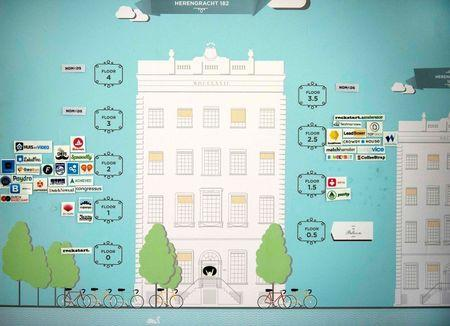
\includegraphics[width=\textwidth]{../immagini/rockstart-building}
\caption{Organizzazione dell'edificio di Rockstart}  
\end{figure}


Rockstart è suddiviso in quattro sezioni principali, ciascuno con il proprio scopo e modalità operative:

\begin{itemize}

\item \textbf{Rockstart accelerator}, che fornisce un programma di accelerazione di 150 giorni, offrendo inoltre un finanziamento iniziale in cambio di una percentuale di quota societaria. Esso si suddivide a sua volta in due sotto-branchie:

\begin{itemize}

\item \textbf{Web e mobile accelerator program}, focalizzato sulle start up in ambito web/mobile. È esattamente in questa branchia in cui l'azienda CoffeeStrap colloca la propria posizione all'interno di Rockstart;

\item \textbf{Smart energy}, che fornisce supporto nelle start-up che mettono in correlazione l'\textit{information technology} con il problema del risparmio energetico. Il loro programma differisce leggermente rispetto al precedente.

\end{itemize}

\item \textbf{Rockstart spaces}, che si occupa della gestione degli uffici e degli eventi all'interno di Rockstart. Quest'ultimo ospita infatti al suo interno numerosi eventi nella spaziosa \textbf{ballroom}, molto spesso organizzati da entità al di fuori di Rockstart;

\item \textbf{Rockstart answers}, che organizza eventi mirati a creare una sorta di comunità all'interno di Rockstart nella quale tutti possono confrontarsi tra di loro ed incontrarsi ad eventi organizzati \textit{ad-hoc} che trattano diversi argomenti o danno la possibilità alle start-up di effettuare presentazioni;

\item \textbf{Rockstart impact}, che fornisce supporto alle start-up nei paesi in via di sviluppo, in particolare in Nepal. 

\end{itemize}

\begin{figure}[htp]
\centering
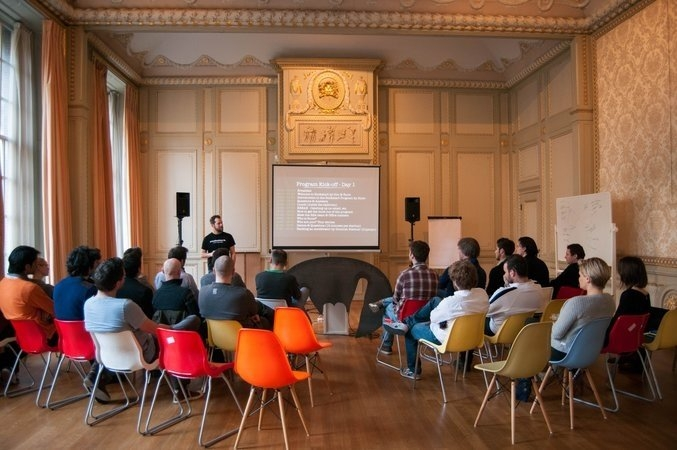
\includegraphics[width=\textwidth]{../immagini/rockstart-ballroom}
\caption{La ballroom a Rockstart}  
\end{figure}

\subsection{Il contesto della start-up}

L'azienda ospitante è una particolare realtà aziendale, l'impresa è nella sua fase iniziale e, come la maggior parte delle start-up, parte con un'idea di riferimento, cercando di rendere profittevole quest'ultima tramite veloci iterazioni sul prodotto. L'incubatore all'interno del quale lavoravo incapsula questo mondo in maniera molto significativa. Sono entrato in un ambiente molto personalizzante, nel quale si è a stretto contatto con il team (essendo quest'ultimo inoltre di piccole dimensioni) e le altre aziende, con le quali si è creata un'implicita rete collaborativa, dalla quale è possibile imparare molto e confrontarsi quotidianamente. Tale collaborazione fornisce valore al prodotto e all'azienda, in quanto permette, oltre ad un importante feedback sulle iterazioni, anche una quotidiana attività di \gls{brainstorming}, che permette di visualizzare i problemi sotto punti di vista differenti e ad arrivare così ad una migliore soluzione.

\section{Il dominio applicativo}

L'idea di CoffeeStrap è quella di fornire un sistema \gls{peer-to-peer} per l'apprendimento di una lingua straniera tramite interazioni con altre persone che parlano quella determinata lingua. L'intento è quello di creare una comunità di utenti che vogliano imparare una lingua e siano allo stesso tempo disposti a fornire supporto ad altri utenti con le lingue cui sono già fluenti. L'interazione può avvenire tramite \textbf{comunicazione testuale}, in cui viene messa a disposizione una vera e propria \textit{chat}, oppure tramite \textbf{comunicazione audio/video}, in cui gli utenti parlano tra di loro nella lingua concordata. Gli utenti hanno la possibilità di iscriversi tramite email o tramite facebook. Il profilo utente è caratterizzato dai seguenti campi:

\begin{itemize}

\item Nome;
\item Cognome;
\item Età (opzionale);
\item Immagine profilo;
\item Città di provenienza;
\item Lingue conosciute;
\item Lingue da imparare.

\end{itemize}

Una volta completato il profilo l'utente inizia a parlare una lingua passando attraverso un flusso:

\begin{itemize}

\item L'utente $X$ seleziona la lingua $Y$ che vuole praticare;
\item Il sistema cerca all'interno della comunità un sottoinsieme $Z$ di persone che parlano la lingua $Y$ (come lingua madre o seconda lingua);
\item Il sistema notifica quest'ultimo, informando gli utenti che l'utente $X$ vuole praticare la lingua $Y$;
\item Gli utenti del sottoinsieme $Z$ decidono se accettare o meno la richiesta dell'utente $X$ di praticare la lingua $Y$;
\item Se l'utente accetta la richiesta allora viene creato un \textbf{match} tra quest'ultimo e l'utente $X$, ed essi iniziano un'interazione.

\end{itemize}

\begin{figure}[htp]
\centering
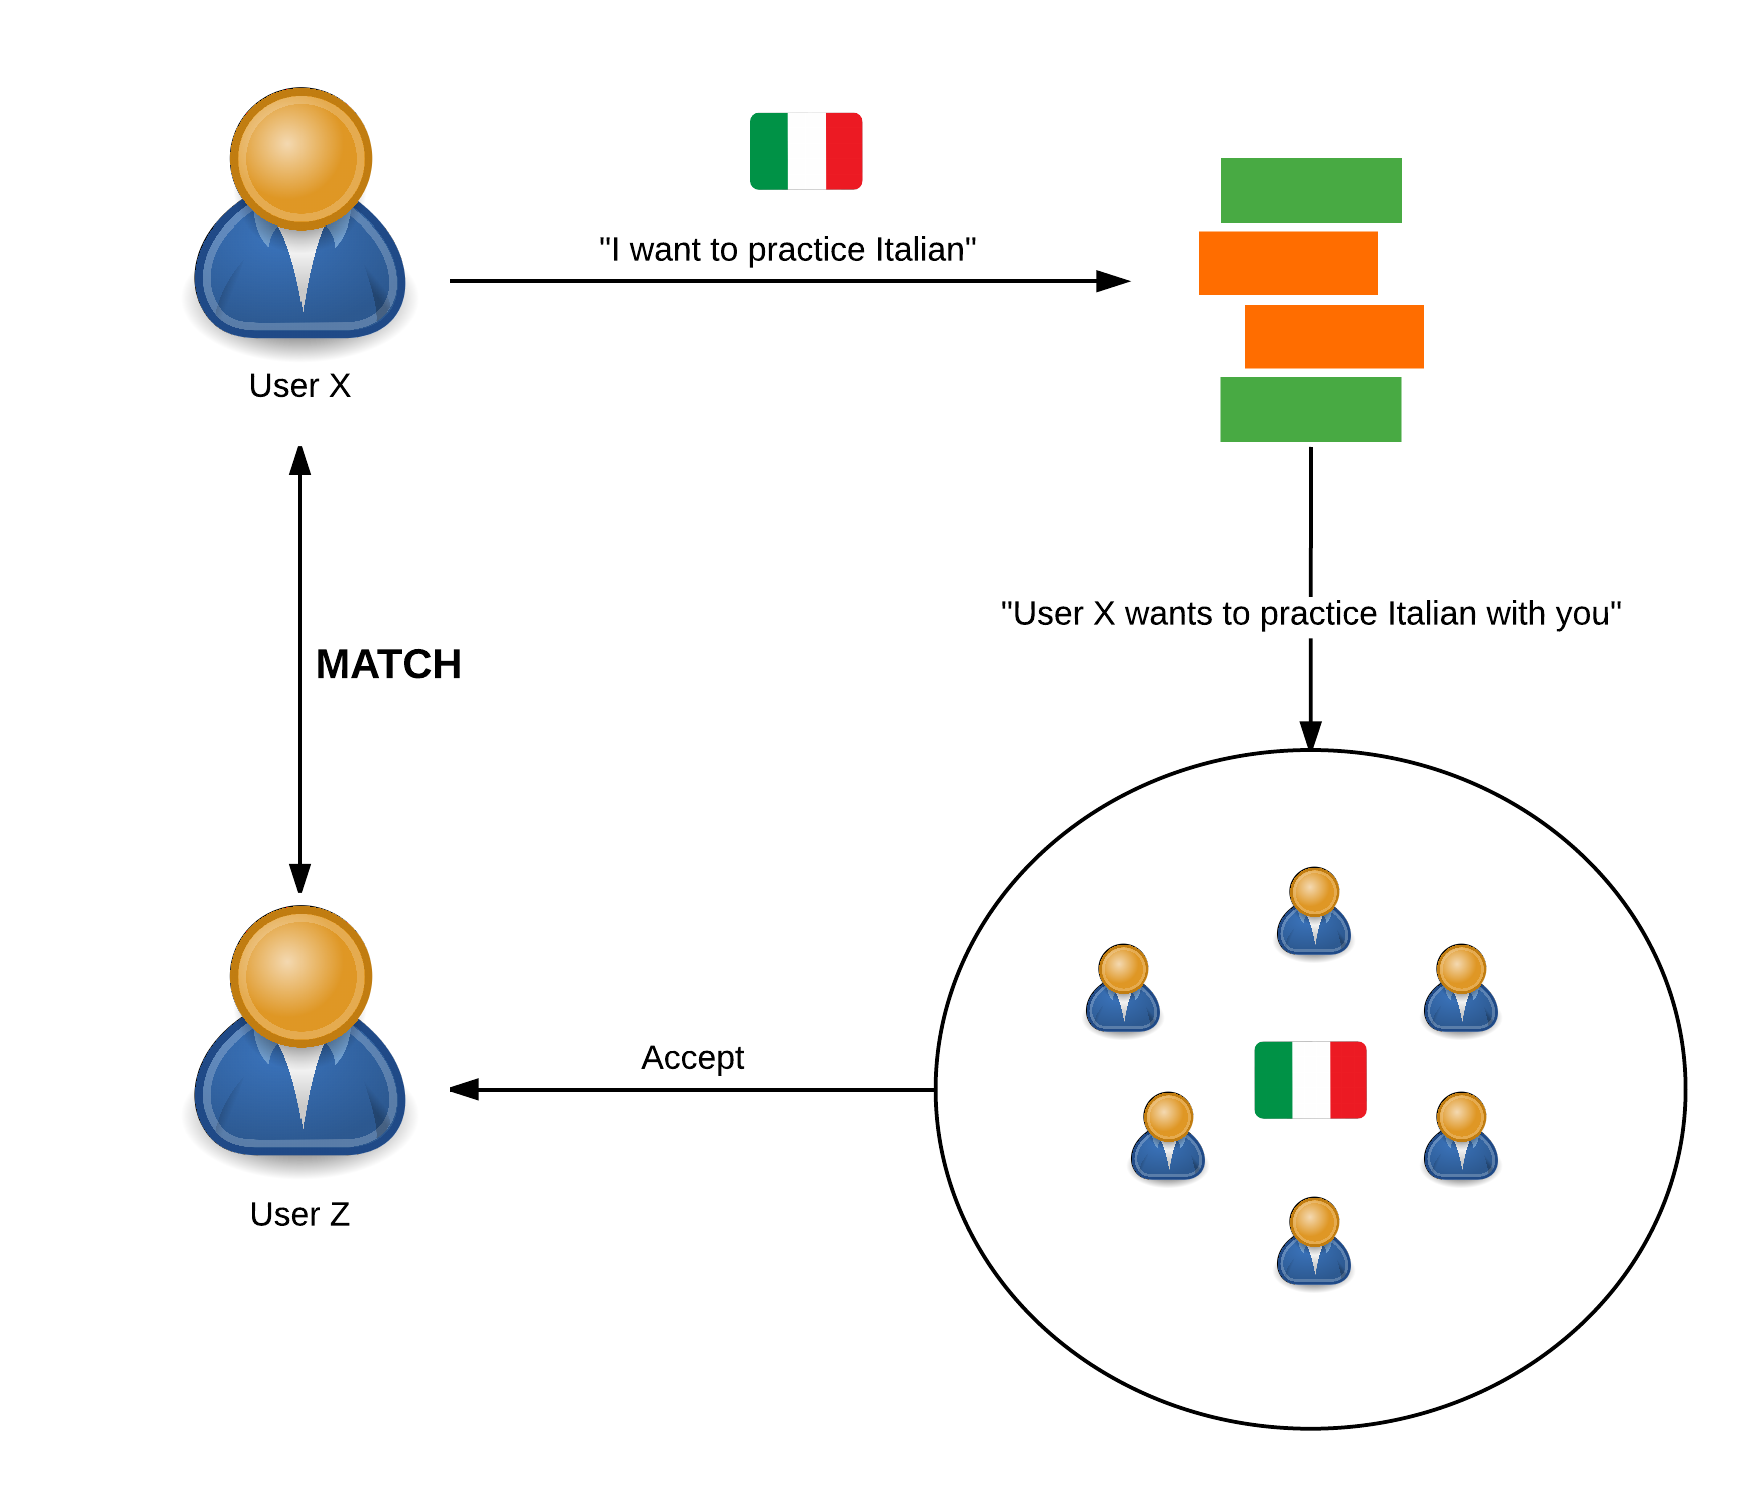
\includegraphics[width=9.75cm]{../immagini/coffeestrap-flow}
\caption{Rappresentazione del flusso utente di CoffeeStrap}
\end{figure}

Gli utenti vengono notificati tramite \textbf{notifica email} e, in seguito allo sviluppo dell'applicazione, \textbf{notifica mobile}.

\section{Metodologie e strumenti di sviluppo}

CoffeeStrap adotta la metodologia di sviluppo \textbf{\gls{agile}}\footnote{\url{http://agilemanifesto.org/}}. Il particolare contesto entro il quale si trova fa sì che i requisiti cambiano molto spesso e porta dunque quest'ultima a dover iterare molto velocemente sul proprio prodotto, che si trova ancora nella sua fase primordiale e necessita di modifiche e miglioramenti costanti. Proprio a fronte di queste necessità è importante mantenere la massima flessibilità possibile nello sviluppo, motivo per cui questo modello di ciclo di vita è in questo momento il più conveniente in termini di efficienza ed efficacia. In particolare la metodologia adottata è quella \textbf{agile \gls{scrum}}.

Il tipo di iterazione utilizzata è su base settimanale. Una volta a settimana, normalmente il Mercoledì, avviene lo \textbf{scrum meeting}, una riunione della durata di circa due ore nella quale si fissano \textbf{story} da risolvere nello \textbf{\gls{sprint}} corrente. Una story è un concetto molto simile a quello di \textbf{ticket}, ed è composta dai seguenti campi:

\begin{itemize}

\item \textbf{Titolo};
\item \textbf{Tipologia}, che può assumere i seguenti valori:

	\begin{itemize}

	\item \textbf{Feature}, quando c'è da aggiungere un ``pezzo'' al sistema;
	\item \textbf{Bug}, quando c'è da risolvere una problematica all'interno del sistema;
	\item \textbf{Chore}, quando c'è da eseguire \textit{refactoring} e manutenzione del codice;
	\item \textbf{Release}, sono marcatori di \textit{milestone} che tracciano il progresso del team rispetto agli obiettivi.

	\end{itemize}

\item \textbf{Descrizione}, che fornisce una dettagliata sintesi della story.
\item Una o più \textbf{etichette}, che forniscono un filtro;
\item \textbf{Complessità}, che è un indice soggettivo di quante risorse sono necessarie per il completamento della story. Questo valore segue la sequenza di Fibonacci e può assumere i valori 1, 2, 5, 8, 13. Se una story ha una complessità superiore a 13 essa dev'essere necessariamente spezzata in due o più sotto-story. Solamente alle features può essere assegnata complessità, in quanto sono le uniche story che realmente forniscono un valore al business;
\item \textbf{Richiedente}, che dev'essere unico;
\item Uno o più \textbf{responsabili} (\textit{owners}), che possono coincidere con il richiedente e sono coloro che devono occuparsi direttamente della story;

\end{itemize}

Opzionalmente inoltre è possibile aggiungere alla story dei tasks, in modo da dividere ulteriormente il lavoro. Ciononostante su di essi non vi è alcun controllo, in quanto il loro utilizzo è a discrezione dei responsabili.

\begin{center}
\begin{table}[htpd]
  \begin{tabularx}{\textwidth}{ | c | X |}
    \hline
    \textbf{Titolo} & Login/registrazione con Facebook \\
    \hline
    \textbf{Tipologia} & Feature \\
    \hline
    \textbf{Descrizione} & È necessario interfacciarsi con le API di facebook per Android per poter implementare il sistema di login/registrazione tramite facebook. Una volta ottenuto il token di accesso l'applicazione deve effettuare una chiamata API a CoffeeStrap fornendo quest'ultimo e memorizzando il cookie restituito dalla chiamata. \\
    \hline
    \textbf{Etichette} & \texttt{Mobile} \\
    \hline
    \textbf{Complessità} & 8 \\
    \hline
    \textbf{Richiedente} & Alessandro Maccagnan \\
    \hline
    \textbf{Responsabili} & Luca De Franceschi \\
    \hline
  \end{tabularx}
  \caption{Un esempio di story}
 \end{table}
\end{center}

Ciascuna story è inserita all'interno di una \textbf{board}. Ci sono tre tipologie di board:

\begin{itemize}

\item \textbf{Current}, contenente le story attive nello sprint corrente;
\item \textbf{Backlog}, contenente la ``coda'' delle story da attivare;
\item \textbf{Icebox}, contente story in attesa di approvazione e attivazione. Le story possono rimanere su questa board per un tempo indeterminato, finché vengono spostate sul backlog o rimosse definitivamente.

\end{itemize} 

A ciascun membro del team vengono assegnate una o più story, la cui scadenza è lo scrum meeting successivo. A quest'ultimo viene richiesto inoltre di assegnare la complessità a quella story, la quale dovrà essere calcolata secondo criteri derivati dalla propria esperienza di sviluppo. Ogni story dev'essere analizzata, progettata, sviluppata e infine testata. La chiusura della story viene effettuata solamente al seguito di una verifica e validazione da parte del responsabile e del richiedente o, se il richiedente coincide con il responsabile, da un altro membro del team. In generale i responsabili non possono approvare le proprie story.

Una volta creata la story deve passare attraverso diverse fasi, per questo si parla di \textbf{story workflow}:

\begin{enumerate}

\item La story viene \textbf{creata} e \textbf{definita} (\textit{define and design});
\item I responsabili assegnano loro una \textbf{stima di complessità}, che va generalmente discussa all'interno del team (\textit{estimate});
\item La story viene \textbf{attivata}: da questo momento i responsabili possono procedere allo sviluppo (\textit{start});
\item La story una volta implementata viene \textbf{testata} (\textit{test});
\item Superata la fase di testing la story viene \textbf{ultimata} (\textit{finish});
\item A questo punto i responsabili ``pushano'' il codice sull'ambiente di \textbf{staging} (\textit{deliver});
\item La story viene poi \textbf{accettata} dal richiedente o comunque da una persona esterna al gruppo di responsabili e viene effettuato il pushing sull'ambiente di \textbf{production} (\textit{accept}). Se la story non viene accettata si itera dal punto 4;
\item Infine, se la story è stata accettata avviene il suo \textbf{rilascio}, che coincide con la terminazione del suo ciclo di vita (\textit{release}).

\end{enumerate}

\begin{figure}[htpd]
\centering
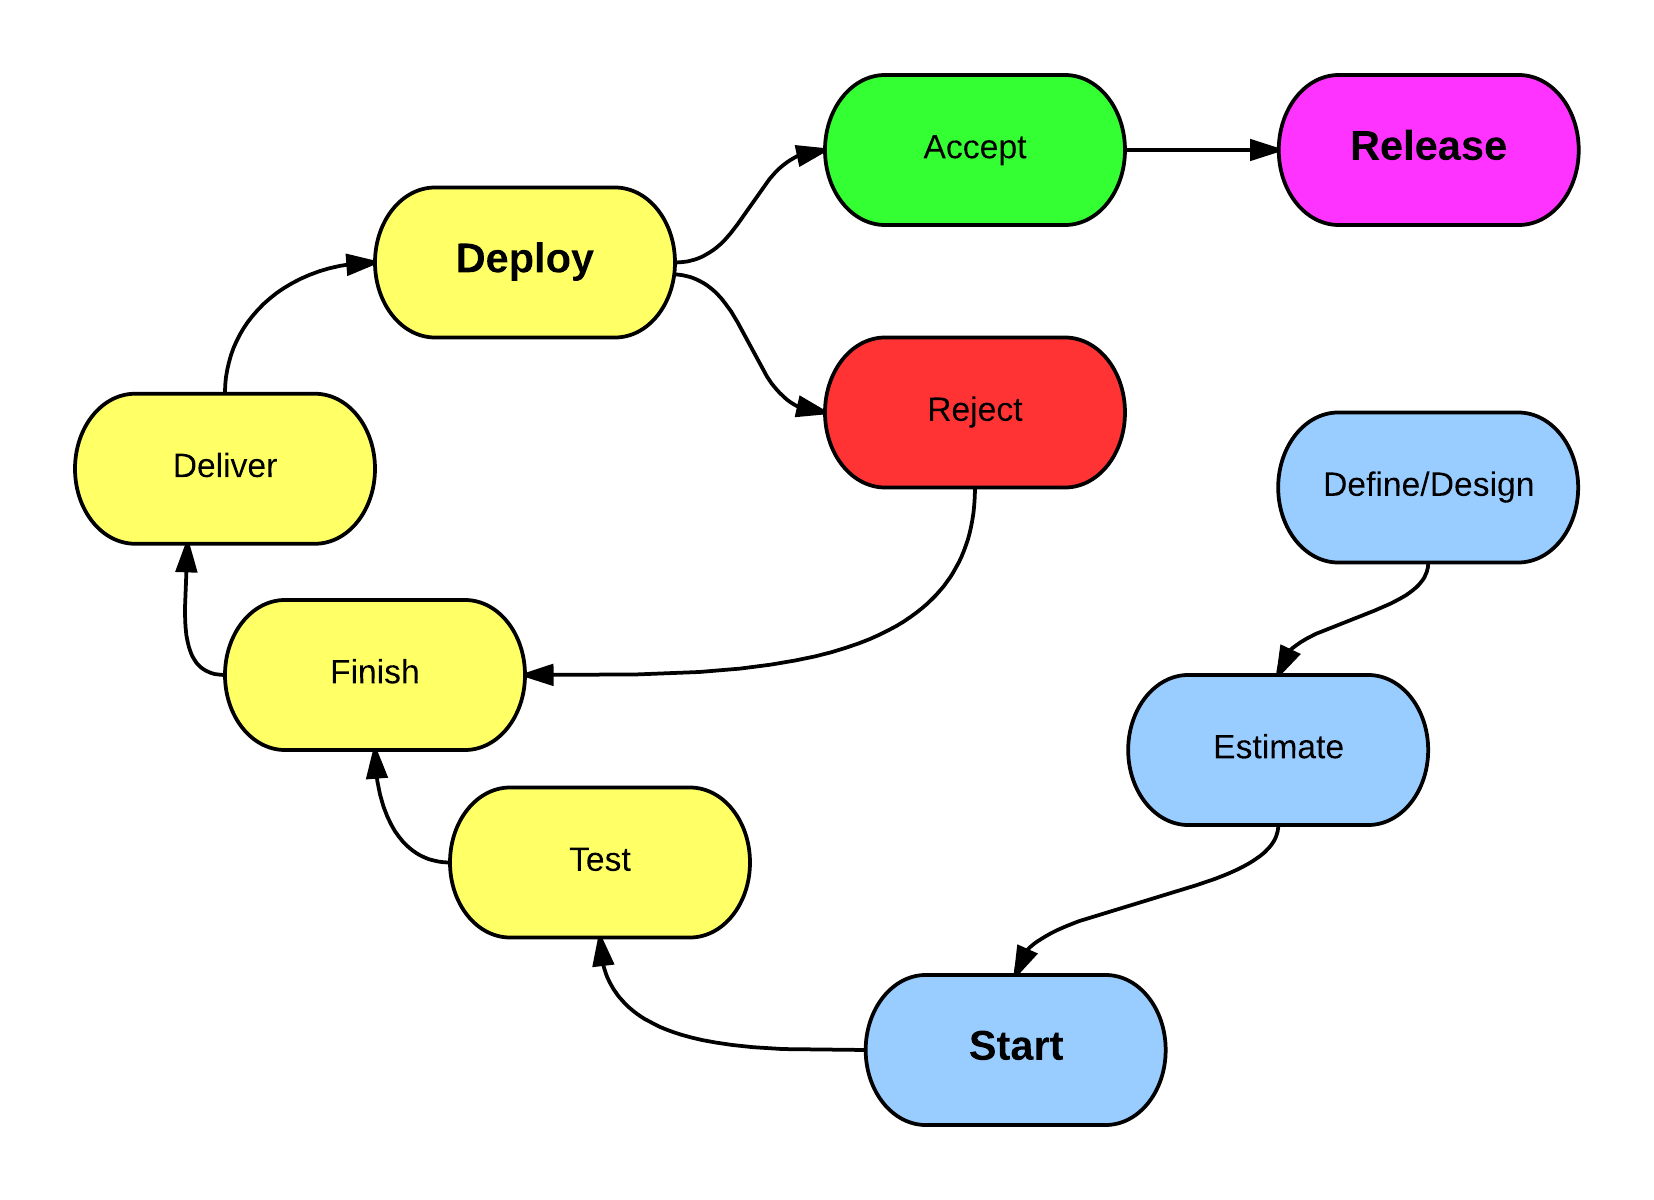
\includegraphics[width=\textwidth]{../immagini/story-workflow}
\caption{Il flusso di una story}
\end{figure}

Alla fine dello sprint viene tracciata la somma delle complessità di tutte le story assegnate a tutti i membri e che sono state chiuse nello sprint corrente. Tale somma è detta \textbf{velocity}, ed è un indice di efficienza di sviluppo dello sprint, che va confrontato con gli sprint precedenti.

Oltre allo scrum meeting viene instanziato quotidianamente lo \textbf{stand-up meeting}, detto anche \textbf{daily scrum}, nel quale prima dell'inizio della giornata lavorativa si effettua una breve riunione con il team, in cui ciascuno espone quanto fatto nel giorno precedente e ciò che ha in programma di fare nel giorno corrente. Quest'attività è di fondamentale importanza per \textbf{monitorare} il progresso dello sprint e sollevare eventuali difficoltà riscontrate nello svolgimento della story. 

\section{Tecnologie}

\subsection{Back-end}

Il back-end è composto da un server scritto tramite il framework \gls{Node.js}\footnote{\url{http://nodejs.org/}}. Questa scelta è dovuta alla necessità di ottimizzare i tempi di produzione e manutenzione del software e la grande potenza e scalabilità di quest'ultimo viene incontro a questo bisogno. La \textbf{programmazione asincrona} e il motore \textit{JavascriptV8} garantiscono una velocità di trasmissione molto elevata e le applicazioni web scritte con \textit{express.js}\footnote{\url{http://expressjs.com/}} sono in grado di reggere un alto carico di lavoro, sostenendo centinaia se non migliaia di richieste simultanee su macchine che non hanno a disposizione molte risorse di memoria. Inoltre Node.js è un linguaggio di programmazione all'avanguardia, in costante aggiornamento, la cui comunità è in forte espansione. Tramite \textbf{npm}\footnote{\url{https://www.npmjs.com/}}, gestore di pacchetti per Node.js, è possibile attingere ad una vasta quantità di librerie utili per ogni evenienza.

Il server fornisce tutta una serie completa di \textbf{\gls{API} \gls{REST}ful} accessibili dall'esterno, alcune delle quali richiedono autenticazione. Ciò permette a tutti i client che si interfacciano con esso, in particolare l'applicazione web e l'applicazione mobile, di poter comunicare con esso in modo semplice e lineare, dovendo riferirsi solamente alle specifiche di queste ultime ed utilizzando una libreria per la gestione delle chiamate API. 

Parallelamente al server è stato instanziato un servizio di \textbf{pushing} fornito da \textbf{firebase}\footnote{\url{https://www.firebase.com/}}, un \textbf{\gls{Cloud Service Provider}} utilizzato per il sistema di notifiche e per fornire un punto d'accesso centralizzato dal quale i diversi componenti (intesi come componenti software) possono comunicare. Firebase fornisce infatti un \textbf{database in tempo reale}, con il quale è possibile interagire e ``\textit{mettersi in ascolto}'' degli eventi su di esso. Esso fornisce un'API pubblica per diversi stack tecnologici e piattaforme.

\subsection{Front-end}

Il front-end è composto da un'applicazione web scritta con \textbf{\gls{Angular.js}}\footnote{\url{https://angularjs.org/}} e \textbf{\gls{HTML5}}, utilizzando il framework CSS \textbf{\gls{Bootstrap}}\footnote{\url{http://getbootstrap.com/}}. Tramite Angular.js è possibile interfacciarsi alle API fornite dal back-end in maniera molto efficiente e popolare dunque le pagine in base alle risposte provenienti da esso. Inoltre, analogamente ad \textit{npm}, per lo sviluppo di applicazioni con Angular.js è disponibile \textbf{bower}\footnote{\url{http://bower.io/}}, gestore di pacchetti per quest'ultimo.

\subsection{Database}

CoffeeStrap utilizza \textbf{\gls{MongoDB}}\footnote{\url{http://www.mongodb.org/}} come database documentale di riferimento. Questa scelta è dovuta alla grande flessibilità offerta dai database di questo tipo, oltre al fatto che negli ultimi mesi è divenuto molto popolare nella comunità di sviluppatori e presenta prestazioni notevoli. 

Dal momento che i requisiti cambiano molto rapidamente è necessario avvalersi di strumenti che siano il più flessibili possibili ai cambiamenti, e MongoDB risponde perfettamente a questo tipo di esigenza. Inoltre MongoDB presenta un facile approccio al suo utilizzo sia per l'utilizzo da parte dello sviluppatore che in termini di scalabilità.

\begin{figure}[htpd]
\centering
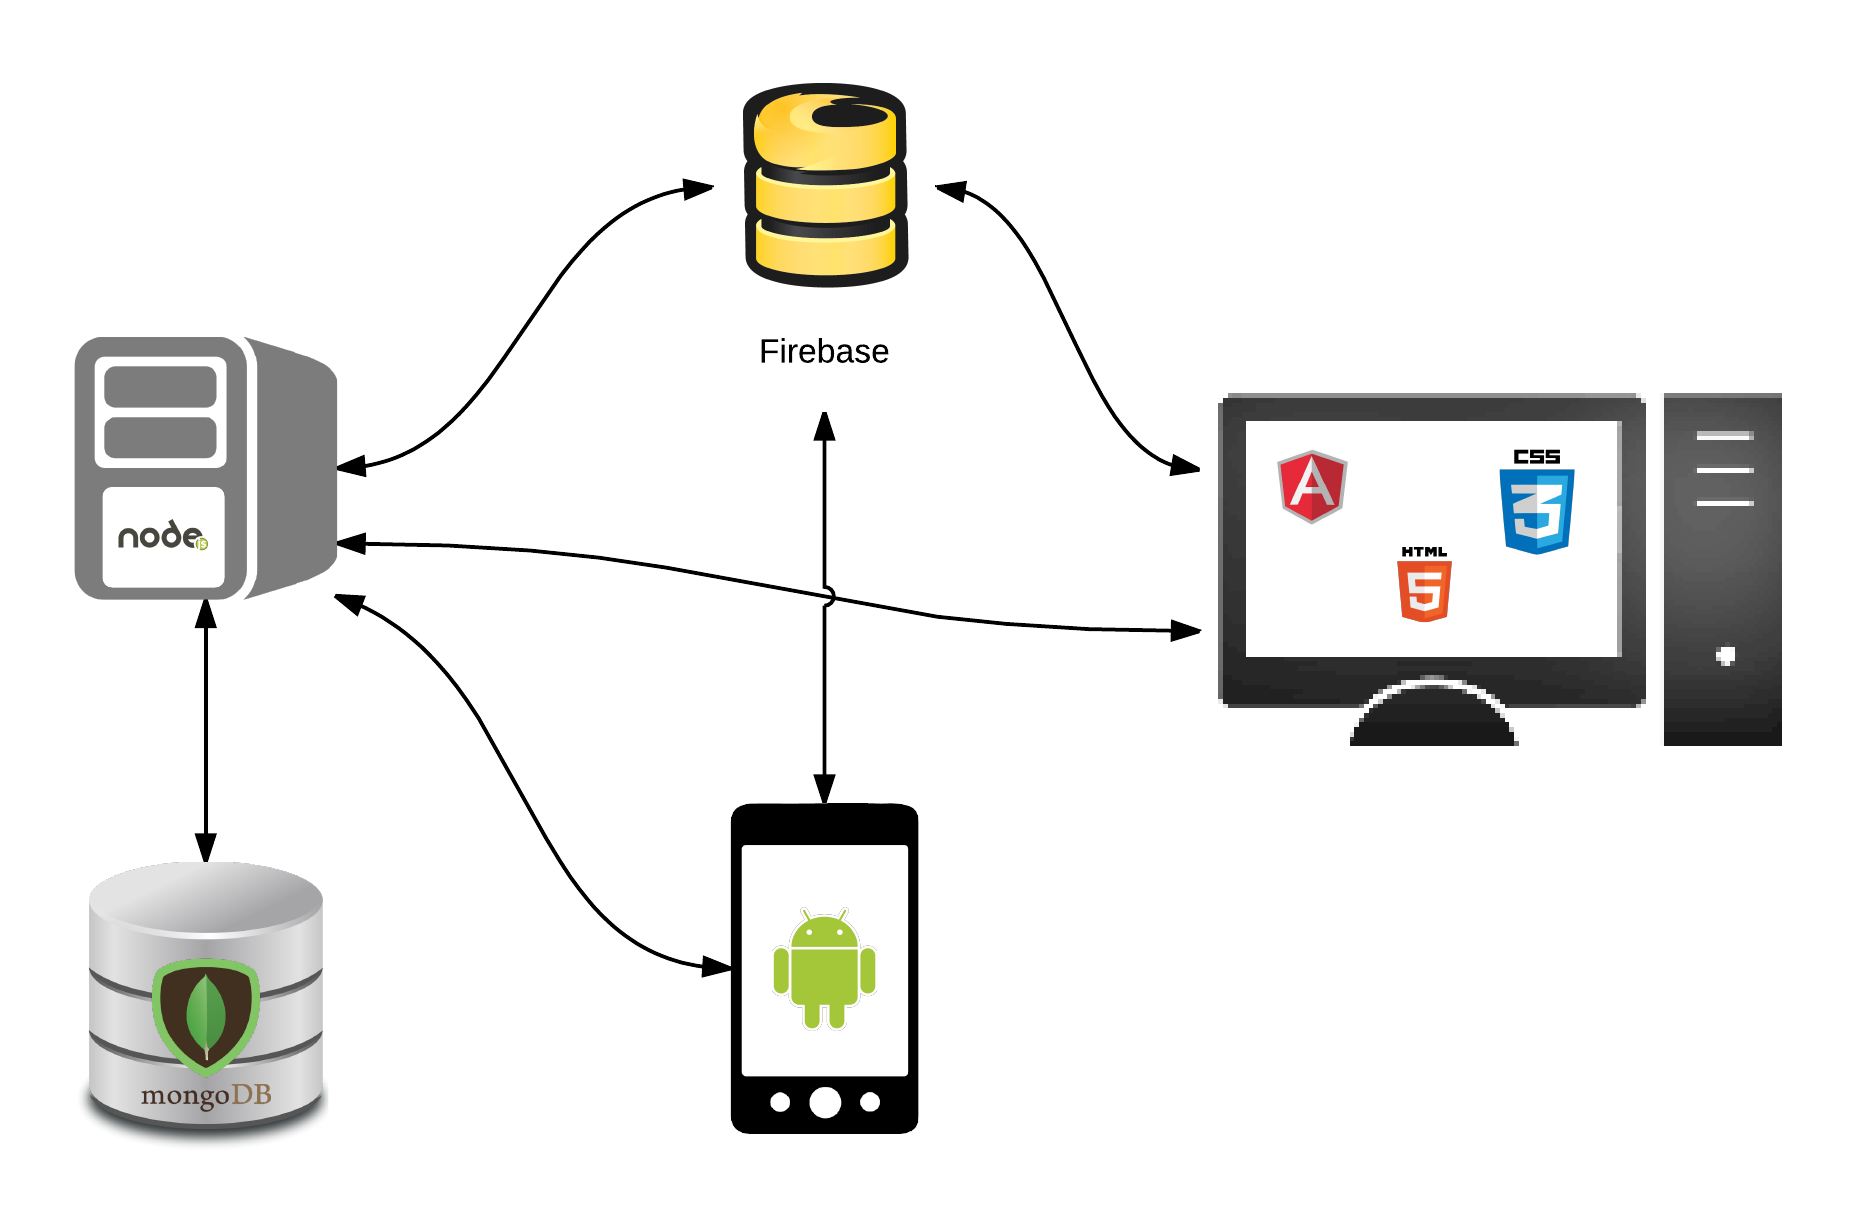
\includegraphics[width=\textwidth]{../immagini/stack-composition}
\caption{Composizione della tecnologia adottata da CoffeeStrap}  
\end{figure}

\subsection{Ambienti di sviluppo}

All'interno dell'azienda si delineano principalmente due ambienti di sviluppo:

\begin{itemize}

\item \textbf{Production}, all'interno del quale risiedono le versioni ufficiali del codice esposte pubblicamente agli utenti;

\item \textbf{Staging}, un ambiente riservato esclusivamente al team e che rappresenta una sorta di ``cantiere'', nel quale risiede una versione del codice ancora da verificare, che può quindi essere testata liberamente e non crea danni verso l'esterno.

\end{itemize}

Ciascun ambiente è caratterizzato dalla propria configurazione, possiede il proprio server e il proprio database ed è agnostico rispetto all'altro.

Occasionalmente è inoltre uso comune instanziare un ambiente ausiliario di sviluppo, per circostanze particolari che necessitano di una configurazione diversa. Solitamente sono ambienti ``\textit{usa e getta}'', che nascono da esigenze particolare e vengono rimossi alla fine del loro utilizzo.

\subsection{Versionamento}

Come strumento di controllo versione del codice sorgente l'azienda utilizza \textbf{\gls{Git}}\footnote{\url{http://git-scm.com/}}, utilizzando \textbf{Bitbucket}\footnote{\url{https://bitbucket.org/}} come servizio di hosting. I motivi che hanno spinto all'utilizzo di Git in luogo di altri sistemi di versionamento sono i seguenti:

\begin{itemize}

\item \textbf{Disponibilità}: ciascun sviluppatore ha una copia locale dell'intero repository ed effettua \textit{\gls{commit}} in locale, potendo dunque lavorare anche in assenza di connessione;

\item \textbf{Semplicità}: oltre ad essere veloce Git permette con facilità la creazione di \textit{branch} e successivi \textit{\gls{merge}}. L'utilizzo di questi ultimi è fondamentale per poter soddisfare il punto seguente:

\item \textbf{Utilizzo di Gitflow}: questo \textbf{workflow} definisce uno stretto modello di \textit{branching} che ruota intorno al progetto. Ciò non aggiunge nuovi concetti o strumenti a Git, ma piuttosto assegna ruoli specifici ai diversi rami. Un approfondimento di questa metodologia è raccolta nell'appendice A.

\end{itemize}

\section{Clientela di riferimento}

CoffeeStrap non ha ancora acquisito finanziamenti da parte di investitori e non presenta associazioni con altre aziende o entità, motivo per cui essi devono rispondere unicamente agli \textbf{utenti finali} del prodotto. Questi ultimi sono persone reali provenienti da ogni parte del mondo, che mettono a disposizione le proprie competenze linguistiche e vogliono allo stesso tempo imparare una lingua straniera entrando in contatto con altri utenti. L'intera struttura di CoffeeStrap si basa su questa \textbf{rete sociale}, composta da un insieme eterogeneo di persone che espongono il proprio profilo all'esterno. È possibile immaginare CoffeeStrap come un vero e proprio \textit{social network} il cui scopo è l'apprendimento linguistico.

\begin{figure}[htpd]
\centering
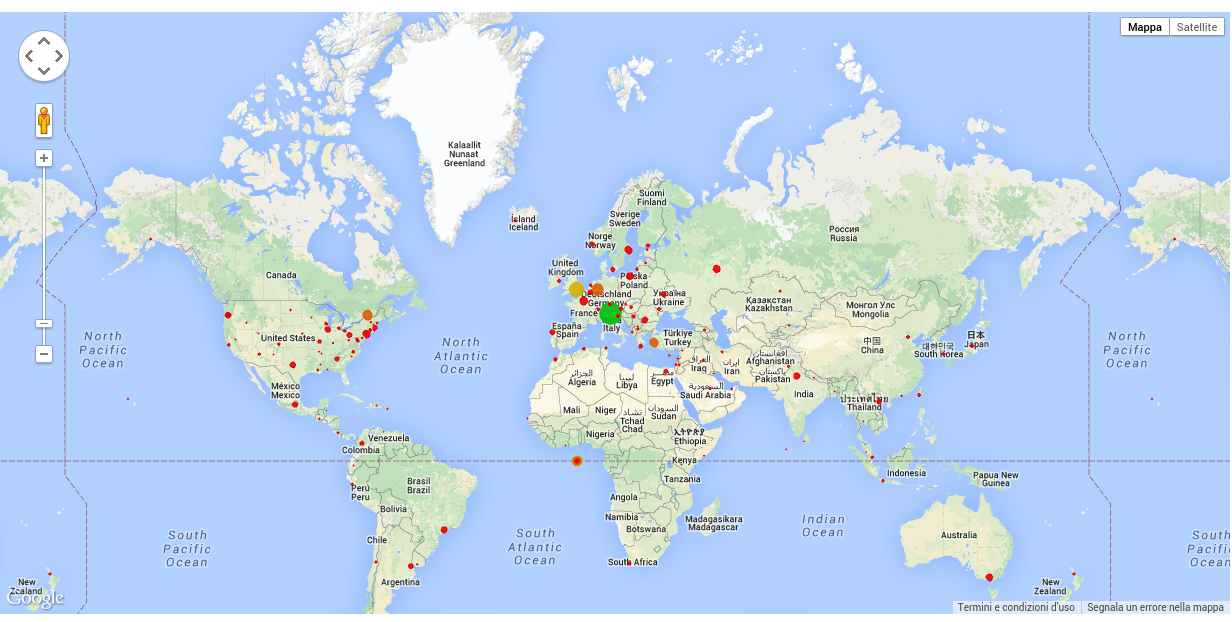
\includegraphics[width=\textwidth]{../immagini/user-distribution}
\caption{Distribuzione degli utenti di CoffeeStrap nel mondo aggiornata a Dicembre 2014}
\end{figure}           
% !TEX encoding = UTF-8
% !TEX TS-program = pdflatex
% !TEX root = ../tesi.tex
% !TEX spellcheck = it-IT

%**************************************************************
\chapter{Framework analizzati}
\label{cap:framework-analizzati}
%**************************************************************
Questo capitolo inizia con una descrizione generale della tipologia di framework analizzati, per poi andare a descrive più in dettaglio il funzionamento dei singoli framewrok, seguito da una sintesi dei pregi e difetti e un breve resoconto riguardo il prototipo realizzato.
Infatti, per valutare al meglio ogni framework è stato realizzata un'applicazione prototipo che visualizza una gallery di immagini ottenuta mediante chiamate ad \gls{API} \gls{REST}.\\
La struttura del prototipo è stata scelta in modo tale da verificare le seguenti caratteristiche:
\begin{itemize}
\item possibilità di disporre le immagini in una griglia;
\item possibilità di implementare lo scroll infinito, una tecnica per ottimizzare il caricamento di grandi quantità di dati che prevede il caricamento iniziale di un limitato numero di elementi, per poi caricare gli elementi rimanenti man mano che l'utente prosegue nella visualizzazione dei dati.
\item fluidità dell'applicazione, specialmente durante il caricamento dei dati;
\item possibilità di personalizzare la barra di navigazione dell'applicazione.
\end{itemize}

\todo[inline]{Valutare se inserire le informazioni riguardo l'esecuzione di un'applicazione}

\section{Considerazioni generali}
Le applicazioni realizzate con questa tipologia di framework hanno alla base lo stesso funzionamento: una \gls{virtual machine} interpreta il codice JavaScript e utilizza un componente ``\textit{ponte}'' per modificare l'interfaccia grafica dell'applicazione, la quale è realizzata con i componenti offerti dal \gls{SDK} nativo.

Ognuno dei framework analizzati utilizza un ``\textit{ponte}'' diverso, il cui funzionamento verrà descritto più in dettaglio nell'apposita sezione.

Un'altra caratteristica di questa tipologia di framework è l'assenza del \gls{DOM}.
Infatti, l'interfaccia di un'applicazione di questo tipo è composta da componenti grafici del sistema operativo che vengono creati e composti a durante l'esecuzione dell'applicazione e non da elementi HTML come nelle applicazioni ibride.

Nel complesso si ottengono due grossi vantaggi:
\begin{itemize}
\item l'esecuzione del codice JavaScript e il \gls{rendering} dell'interfaccia grafica avvengono su due thread distinti, rendendo l'applicazione più fluida;
\item utilizzando i componenti grafici nativi si ottiene un esperienza utente più simile a quella che si ottiene con un'applicazione realizzata in \gls{Obj-C}/Java.
\end{itemize}

\subsection{Differenze con le applicazioni ibride}

Un'applicazione ibrida consiste in un'applicazione nativa composta da una \gls{WebView} che visualizza un'insieme di pagine web realizzate utilizzando HTML5, CSS3 e JavaScript, che replicano l'aspetto di un'applicazione nativa.

Trattandosi quindi di un'applicazione web è possibile utilizzare tutti i framework e le tecnologie disponibili nell'ambito web, come AngularJS o jQuery.

Inoltre, se è già disponibile un'applicazione web per desktop, la creazione di un'applicazione mobile ibrida risulta rapida in quanto è possibile riutilizzare sia parte del codice, sia le competenze legato allo sviluppo web dei vari sviluppatori.

Questo approccio viene utilizzato da qualche anno e permette di creare applicazioni che possono accedere ad alcune funzionalità hardware del dispositivo come il giroscopio o la fotocamera e che possono essere commercializzate nei vari store online.

Per supportare questo processo di sviluppo sono stati sviluppati dei framework come Cordova/\gls{PhoneGap} che si occupano di gestire la WebView e di fornire un sistema di plug-in per accedere alle funzionalità native.

Questa tipologia di applicazioni ha però delle limitazioni riguardanti:
\begin{itemize}
\item \textbf{Prestazioni:} trattandosi di una pagina web renderizzata all'interno di un browser, non è possibile sfruttare al massimo le potenzialità della piattaforma sottostante, come il multi-threading. Questo comporta che il codice JavaScript e il rendering dell'interfaccia grafica vengano eseguiti nello stesso thread, ottenendo così un'interfaccia poco fluida.
\item \textbf{Esperienza d'uso:} una delle caratteristiche principali delle applicazioni native sono le \gls{gesture}, l'utente è abituato ad interagire con le applicazioni native, le quali sono dotate di un complessio sistema di riconoscimento delle gesture che non è ancora replicabile in ambito web.
\item \textbf{Funzionalità:} non tutte le funzionalità che può sfruttare un'applicazione nativa sono disponibili in un'applicazione ibrida.
\end{itemize}

Il funzionamento dei framework analizzati in questo capitolo permette di risolvere i problemi principali delle applicazioni ibride, in quanto sfruttando i componenti nativi, non sono presenti i problemi prestazionali legati al rendering dell'interfaccia grafica, il quale non viene bloccato dall'esecuzione del codice JavaScript. Inoltre, sempre per il fatto che  vengono utilizzati componenti nativi, è possibile sfruttare lo stesso sistema di riconoscimento delle gesture e le stesse animazioni, rendendo l'esperienza d'uso più simile a quella offerta da un'applicazione realizzata con l'SDK nativo.

\section{Tabris.js}

Framework pubblicato da EclipseSource\footnote{\url{http://eclipsesource.com/en/home/}} nel Maggio 2014, che permette di controllare mediante JavaScript i componenti dell'interfaccia grafica nativa, sia di iOS, sia di Android.

\subsection{Come funziona}
Tabris.js funziona utilizzando come "\textit{ponte}" una versione modificata di Cordova, la quale, grazie a dei plug-in sviluppati da EcplipseSoruce, permette di interagire via JavaScript con i componenti nativi del sistema operativo.

Ognuno di questi plug-in incapsula un determinato componente dell'interfaccia grafica e fornisce delle API JavaScript per controllarlo.

Trattandosi di un framework derivato da Cordova è possibile utilizzare i plug-in di Cordova già esistenti per aggiungere nuove funzionalità, oltre  a quelle offerte framework, come per esempio l'utilizzo della fotocamera. 

L'unica condizione per il corretto funzionamento dei plug-in esterni è che non dipendano dal DOM, dal momento che il DOM non è presente durante l'esecuzione di un'applicazione.

Il framework viene pubblicato come open source, tuttavia per accedere al codice sorgente è necessario acquistare una licenza, pertanto non è stato possibile analizzare più in dettaglio il funzionamento del framework.

\subsection{Pregi e difetti}

Uno dei pregi di Tabris.js è quello che il codice JavaScript scritto è indipendente dalla piattaforma, questo permette di utilizzare lo stesso codice sorgente e lo stesso layout sia per iOS sia per Android.
\`E il framework che si occupa di eseguire tutte le operazioni specifiche per le varie piattaforme e di renderizzare gli opportuni componenti grafici.

Un altro pregio deriva dall'estensibilità, è infatti possibile utilizzare sia dei plug-in di Cordova, sia i moduli disponibili su \gls{npm}, con la condizione che questi non dipendano dal DOM.

Le criticità di Tabris.js riguardano per lo più il layout che deve essere fatto in modo imperativo, definendo prima la dimensione e la posizione dei vari componenti, per poi organizzarli in modo gerarchico.

Sempre per quanto riguarda il layout, la personalizzazione è limitata in quanto risulta complesso, se non impossibile, definire dei componenti grafici composti o con layout particolari, come la visualizzazione a griglia.

Infine, il framework non impone né suggerisce alcun pattern architetturale da adottare, lasciando completa libertà al programmatore, con il rischio che il codice sorgente dell'applicazione diventi complesso e difficile da manutenere.

\subsection{Prototipo}

\begin{figure}[htp]
\centering
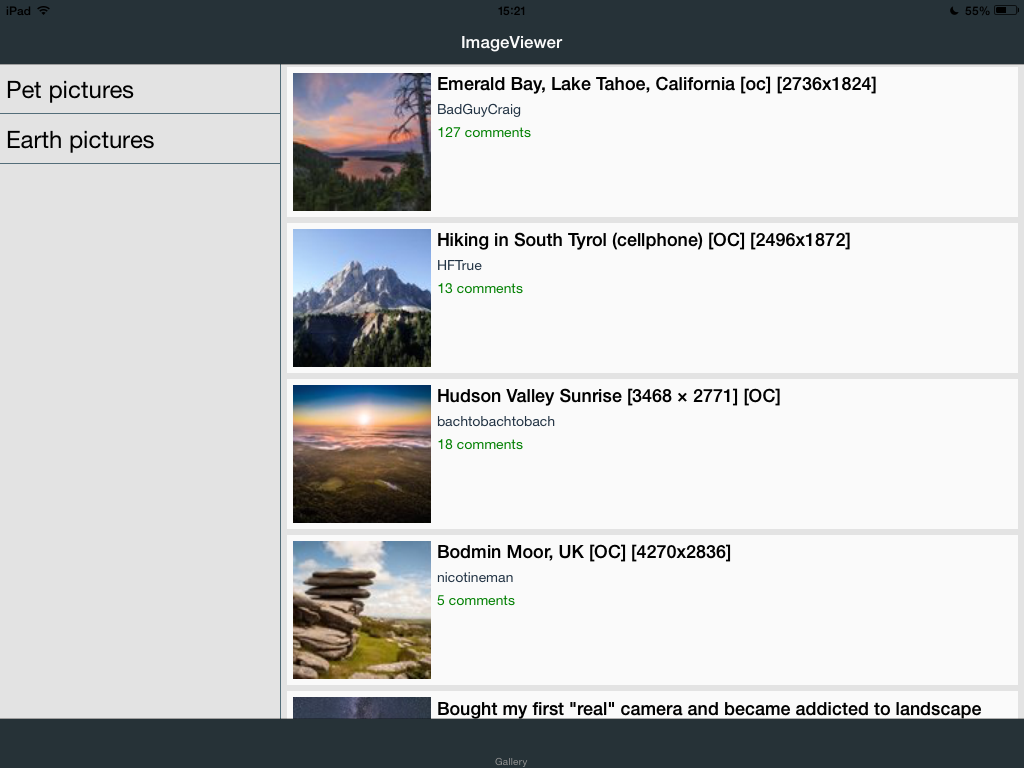
\includegraphics[width=\textwidth]{../immagini/prototipo-tabris}
\caption{Screenshot del prototipo realizzato con Tabris.js}  
\end{figure}

Nel realizzare l'applicazione prototipo sono state riscontrate varie problematiche in particolare riguardanti il layout.
Ad esempio, non è stato possibile disporre gli elementi in una griglia e la personalizzazione della barra di navigazione si è rilevata essere molto limitata.

Un altro problema emerso durante la realizzazione del prototipo è stata la scarsa disponibilità di materiale online, infatti oltre alle risorse messe a disposizione da EclipseSource e alla documentazione ufficiale, non è stato possibile trovare altre informazioni riguardanti il framework.

In ogni caso, l'applicazione realizzata è molto fluida e l'esperienza d'uso è paragonabile a quella di un'applicazione nativa.

\FloatBarrier
\section{NativeScript}

Framework rilasciato da Telerik nel Maggio 2015 che permette di realizzare applicazioni mobile native sia per iOS che per Android rendendo possibile utilizzare tutte le API native mediante JavaScript.

\subsection{Come funziona}

NativeScript utilizza come ``\textit{ponte}'' una virtual machine appositamente modificata che all'occorrenza esegue del codice C++ per invocare le funzioni scritte in linguaggio nativo (Obj-C, Java).

Questa virtual machine deriva da \gls{V8} se l'applicazione viene eseguita su Android o da \gls{JavaScriptCore} nel caso l'applicazione venga eseguita su iOS.

Le modiche subite dalla virtual machine riguardano:
\begin{itemize}
\item la possibilità di intercettare l'esecuzione di una funzione JavaScript ed eseguire in risposta del determinato codice C++;
\item l'iniezione di metadati che descrivono le API native;
\end{itemize} 
In questo modo il runtime di NativeScript può utilizzare i metadati per riconoscere le funzioni JavaScript che hanno una corrispondente funzione nativa, in modo da poter richidere l'esecuzione della funzione nativa mediante del codice C++.

\begin{figure}[htp]
\centering
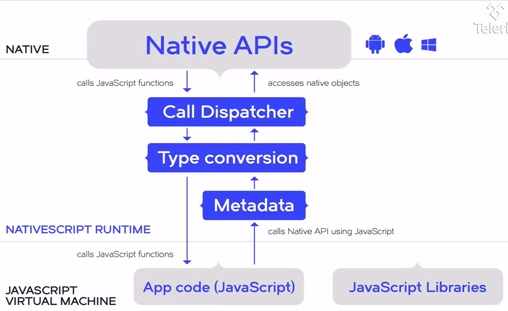
\includegraphics[width=\textwidth*3/4]{../immagini/ns-runtime}
\caption{Schema rappresentante il runtime di NativeScript}  
\end{figure}
\FloatBarrier

Di conseguenza il runtime di NativeScript permette di creare degli oggetti JavaScript che funzionano da \gls{proxy} rispetto agli oggetti nativi specifici della piattaforma.
Un esempio del funzionamento è dato dal seguente codice che su iOS crea un oggetto di tipo \texttt{UIAlertView}:

\begin{lstlisting}[language=JavaScript, caption=Esempio di creazione di un oggetto nativo]
var alert = new UIAlertView();
\end{lstlisting}

All'esecuzione del JavaScript la virtual machine riconosce, grazie ai metadati iniettati, che la funzione JavaScript deve essere eseguita come una funzione nativa.

Di conseguenza, utilizzando del codice C++, invoca la corrispondente funzione Obj-C che in questo caso istanzia un oggetto \texttt{UIAlertView} e memorizza un puntatore all'oggetto nativo in modo da poterlo recuperare in seguito per eseguire delle funzioni su di esso.

Alla fine, la virtual machine crea un oggetto JavaScript che funziona come un proxy dell'oggetto nativo precedentemente creato e lo ritorna in modo che possa essere memorizzato e utilizzato come un normale oggetto JavaScript.

I metadati che vengono iniettati nella virtual machine e che descrivono tutte le funzioni offerte dalle API native della piattaforma, sono ricavati durante il processo di compilazione dell'applicazione utilizzando la proprietà di \gls{riflessione} dei linguaggi di programmazione.

Il vantaggio di questa implementazione è che tutte le API native sono invocabili da JavaScript e anche le future versione delle API potranno essere supportate appena queste vegnono rilasciate.

Inoltre, questi metadati possono essere generati anche per tutte le librerie native di terze parti, rendendole disponibili in JavaScript.

Per permettere il riuso del codice NativeScript fornisce dei moduli che aggiungo un livello di astrazione ulteriore rispetto alle API native, che contiene sia componenti grafici, sia funzionalità comuni ad entrambe le piattaforme, come l'accesso al filesystem o alla rete.
Questo livello di astrazione è opzionale ed è sempre possibile effettuare chiamate dirette alle API native.

\begin{figure}[htp]
\centering
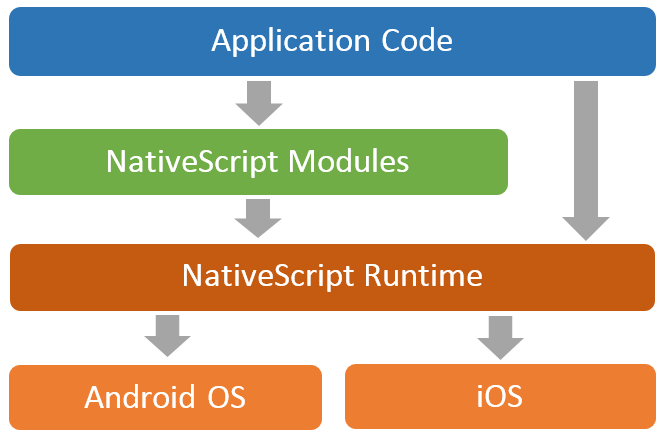
\includegraphics[width=\textwidth/2]{../immagini/ns-architecture}
\caption{Architettura di NativeScript}  
\end{figure}
\FloatBarrier

\subsection{Pregi e difetti}

Il pregio principale di NativeScript è che rende disponibili ad un'applicazione nativa realizzata in JavaScript tutte le funzionalità che possono essere presenti in un'applicazione realizzata con l'SDK nativo. 

Inoltre, l'interfaccia grafica di un'applicazione viene realizzata in modo dichiarativo mediante XML e CSS\footnote{NativeScript implementa un sotto insieme limitato di CSS in quando le istruzioni CSS devono essere applicate sui componenti nativi.}, in un modo analogo a quello utilizzato per le applicazioni web.

Tuttavia, le funzionalità offerte dal livello di astrazione sono limitate e di conseguenza per ottenere effetti particolari è necessario utilizzare le API native.

Questo comporta la diminuzione del codice riusabile su più piattaforme e un notevole aumento della complessità, allontanandosi così dallo scopo principale dell'utilizzo del JavaScript per lo sviluppo di applicazioni native, che è quello di sviluppare in modo semplice e senza utilizzare le API native.

\subsection{Prototipo}

\begin{figure}[htp]
\centering
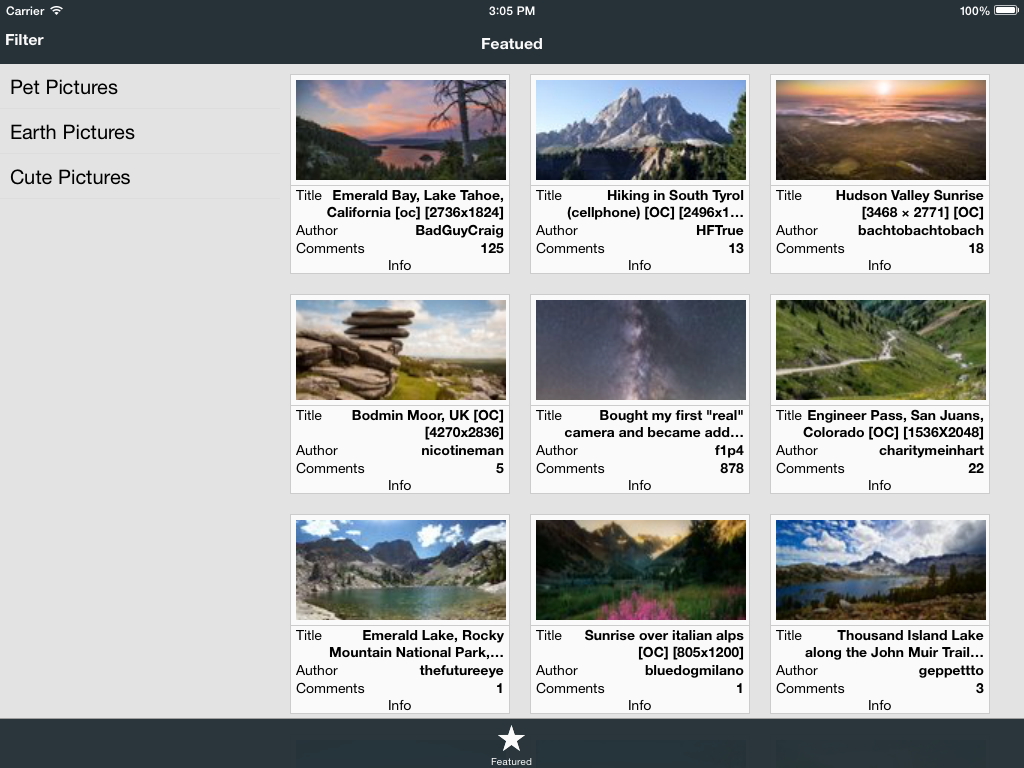
\includegraphics[width=\textwidth]{../immagini/prototipo-react-native}
\caption{Screenshot del prototipo realizzato con NativeScript}  
\end{figure}

Sfruttando quasi solamente i componenti generici offerti da NativeScript è stato possibile ottenere un layout simile a quello dell'applicazione attuale.

Tuttavia per realizzare la visualizzazione a griglia delle immagini è stato necessario utilizzato un componente \texttt{Repeater} all'interno di una \texttt{ScrollView}, questa implementazione risulta poco efficiente e poco fluida, in quanto non essendo mappata su un componente nativo non gode delle stesse ottimizzazioni.

Sono state individuate soluzioni alternative sfruttando librerie native di terze parti, che non sono state adottate in quanto ritenute troppo complesse dal momento che fanno largo uso di codice specifico per iOS.

\FloatBarrier
\section{React Native}

Framework sviluppato da Facebook come progetto interno per la realizzazione di applicazioni native per iOS sfruttando il JavaScript e con un funzionamento analogo a quello di React\footnote{Framework per lo sviluppo di applicazioni web pubblicato da Facebook.}.

React Native è stato successivamente rilasciato come progetto open source nel Marzo 2015.

\subsection{Come funziona}

React Native è composto da una parte scritta in Obj-C e un'altra parte scritta in JavaScript.
La parte realizzata in Obj-C comprende:
\begin{itemize}
\item una serie di classi che definiscono il ``\textit{ponte}'' che permette di alla virtual machine di invocare codice nativo;
\item un'insieme di macro che permettono alle classi Obj-C di esportare dei metodi in modo che questi possano essere invocati dal ``\textit{ponte}'';
\item un'insieme di classi che derivano dai componenti nativi di uso comune e che utilizzano le macro per esportare alcune funzionalità.
\end{itemize}
La parte realizzata in JavaScript consiste in un livello di astrazione, organizzato in moduli, che nascondere l'interazione con le componenti native.

Tra questi moduli si trova la maggior parte dei componenti grafici necessari per la realizzazione di un'interfaccia grafica e per l'accesso ad alcune delle funzionalità del dispositivo, come le notifiche o i servizi di localizzazione. 

\`E inoltre presente il modulo \texttt{NativeModules} che permette di interagire direttamente con il ``\textit{ponte}'' in modo da utilizzare oggetti nativi personalizzati.

Quando viene avvita un'applicazione con React Native, viene eseguito del codice Obj-C che istanzia sia la virtual machine che andrà ad interpretare il JavaScript, sia il ``\textit{ponte}'' tra la virutal machine e il codice nativo.

Durante l'esecuzione del codice JavaScript è possibile richiedere l'esecuzione di codice nativo usando il modulo \texttt{NativeModules}, questo modulo fornisce all'oggetto ``\textit{ponte}'' le informazioni necessarie per permettergli di identificare la porzione di codice nativo da eseguire.
Per poter essere eseguito il codice nativo deve utilizzare le macro fornite da React Native, altrimenti il ``\textit{ponte}'' non riesce ad identificare il metodo da invocare.

Al fine di ottenere prestazioni migliori, la virtual machine che esegue il JavaScript viene eseguita su un thread diverso rispetto a quello che si occupa dell'esecuzione del codice nativo e del rendering dell'interfaccia grafica.

Inoltre, la comunicazione tra questi due thread viene gestita in modo asicrono ed eseguita in blocchi, in questo modo è possibile ridurre le comunicazioni tra i due thread ed evitare che l'interfaccia grafica si blocchi durante l'esecuzione del codice JavaScript.

\subsection{Pregi e difetti}

React Native fornisce un buon livello di astrazione rispetto la piattaforma nativa, dando la possibilità ad uno sviluppatore web di realizzare un'applicazione nativa completa senza conoscere nulla riguardo il funzionamento della piattaforma sotto stante.

A causa di questa astrazione non tutte le funzionalità native sono disponibili, tuttavia è possibile adattare classi Obj-C già esistenti mediante le macro messe a disposizione dal framework, tuttavia questo processo prevede una buona conoscenza del linguaggio Obj-C e della piattaforma sottostante.

Tra gli altri pregi di React Native c'è la community di sviluppatori creatasi attorno al framework, infatti, nonstante si tratti di un framework pubblicato recentemente, si è già creata una community numerosa ed è già possibile trovare dei moduli open source che estendono le funzionalità base del framework.

Infine il flusso di lavoro per lo sviluppo di un'applicazione con React Native risulta molto veloce, in quanto grazie all'utilizzo dei WebSocket, non è necessario eseguire la build dell'applicazione ad ogni modifica del codice sorgente, portando un notevole risparmio di tempo.

\subsection{Prototipo}

\begin{figure}[htp]
\centering
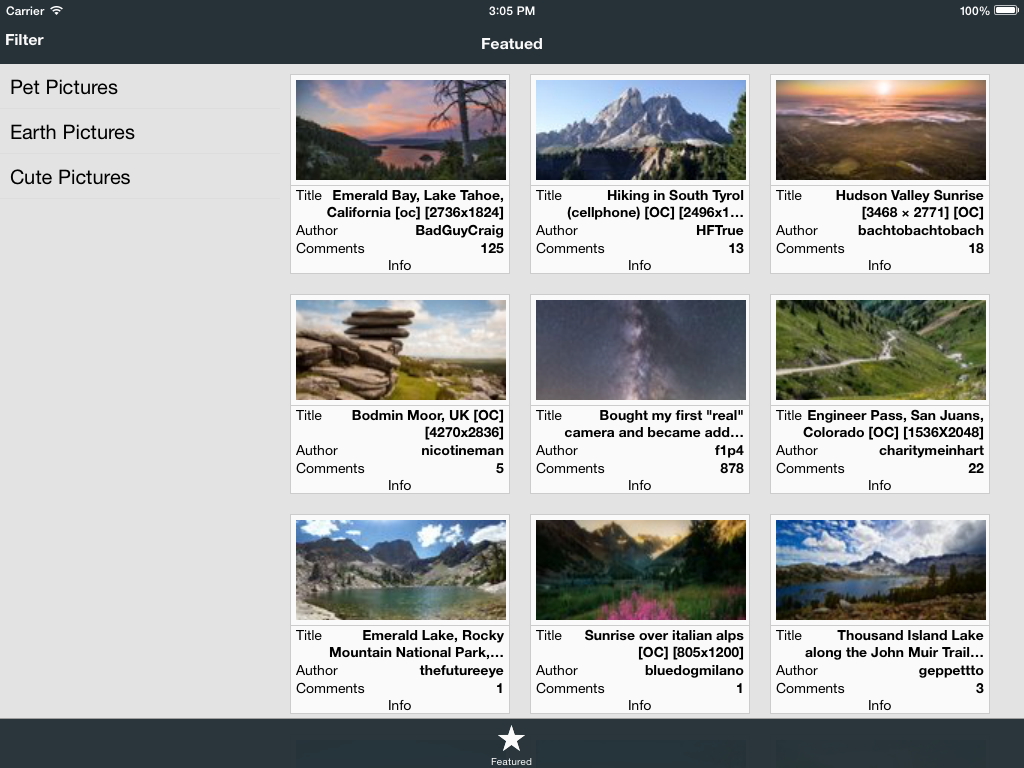
\includegraphics[width=\textwidth]{../immagini/prototipo-react-native}
\caption{Screenshot del prototipo realizzato con React Native}  
\end{figure}

Il prototipo realizzato è stato in grado di soddisfare la maggior parte delle caratteristiche ricercate, infatti è stato possibile ottenere una visualizzazione a griglia, dotata di scroll infinito e fluido.

Sono stati invece incontrati dei problemi riguardanti la personalizzazione della barra di navigazione, in quando il componente offerto dal framework non permette la presenza di pulsanti personalizzati nella barra di navigazione.

Tuttavia sono state individuate alcune soluzioni che prevedono l'utilizzo di moduli open source che forniscono una barra di navigazione maggiormente personalizzabile.

\FloatBarrier
\section{Confronto finale}
\todo[inline]{Trovare un nome migliore}

\begin{table}[h]
\centering

\begin{tabular}{|m{2.3cm}|m{3cm}|m{3cm}|m{3cm}|}
\hline - & Tabris.js & NativeScript & React Native   \\ 
\hline  

Funzionamento & Utilizza dei plug-in di Cordova per rendere accessibili i componenti grafici nativi via JavaScript & Utilizza una VM modificata e dei meta dati relativi alle API native per renderne possibile l'utilizzo via JavaScript  & Utilizza delle classi Obj-C per creare un ponte tra la VM che esegue il JavaScript e le componenti native   \\ 

\hline  

 Possibilità di personalizzazione & Limitata a quanto offerto dal framework & Come se l'applicazione fosse scritta in linguaggio nativo & Limitata a quanto offerto dal framework   \\
 
\hline 

 Estensibilità & Mediante plug-in di Cordova & Mediante librerie native di terze parti & Estendendo librerie native di terze parti con le macro offerte dal framework  \\ 

\hline

 Piattaforme supportate & iOS e Android & iOS e Android & iOS   \\

\hline

\end{tabular}

\caption{Tabella comparativa dei framework analizzati}
\label{my-label}
\end{table}

\FloatBarrier
\section{Framework scelto}

Dopo aver esaminato e confrontato i tre framework individuati si è scelto di utilizzare React Native per la seconda parte dello stage.

Questo perché React Native si è dimostrato un framework molto potente anche se non offre l'accesso completo alle API native come fa NativeScript.
Inoltre, la diffusione già ampia del framework e il supporto da parte di Facebook, che sta attualmente utilizzando React Native per sviluppare alcune delle proprie applicazione, fornisce al framework un'ampia possibilità di crescita, mediante l'estensione di nuove funzionalità o il supporto di ulteriori sistemi operativi, come Android.

Per quanto riguarda NativeScript, è stato scartato principalmente perché non raggiunge l'obiettivo di nascondere la complessità dello sviluppo di un'applicazione nativa con Obj-C o Swift.

Infatti, l'obiettivo che si vuole raggiungere sviluppando un'applicazione nativa in JavaScript è quello di riutilizzare il più possibile le competenze derivate dallo sviluppo web senza dover imparare tutti i dettagli dello sviluppo con l'SDK nativo.

Infine, Tabris.js è stato scartato perché è risultato troppo limitato e non è stato in grado di soddisfare alcune delle caratteristiche ricercate.




             
% !TEX encoding = UTF-8
% !TEX TS-program = pdflatex
% !TEX root = ../tesi.tex
% !TEX spellcheck = it-IT

%**************************************************************
\chapter{Strumenti e tecnologie utilizzate}
\label{cap:strumenti-tecnologie}
%**************************************************************

Il contenuto di questo capitolo contiene una descrizione più dettagliata delle tecnologie e degli strumenti utilizzati per sviluppare l'applicativo oggetto dello stage.

Come anticipato nel precedente capitolo, si è scelto di utilizzare React Native come framework principale per lo sviluppo dell'applicazione, il che vincola la scelta di alcuni strumenti e tecnologie.

\section{React Native}

Trattandosi di un framework per la definizione di interfacce grafiche, React Native prevede di strutturare l'applicazione secondo componenti, ognuno dei quali viene definito combinando componenti standard offerti dalla libreria o altri componenti definiti dallo sviluppatore.
%Visto in un ottica \gls{MVC}, un componente di React Native funziona da \textit{view-controller} in quanto la definizione% di un componente comprende sia la definizione dell'aspetto (\textit{view}), sia la definizione della logica di funzionamento (\textit{controller}). 

React Native offre una serie di componenti basilari che permettono di definire l'interfaccia grafica dell'applicazione e che vengono poi tradotti in componenti nativi. Questi componenti possono essere sia semplici come \texttt{View}, \texttt{Text} o \texttt{Image}, sia più complessi come \texttt{TabBarIOS} o \texttt{MapView}.

%La definizione di un componente di React Native comprende sia la definizione della logica di funzionamento, sia dell'aspetto del componente, il che riportato in un'ottica MVC, fa si che un componente sia un \textit{view-controller}, in quanto funzione sia da \textit{view} che da  \textit{controller}.

Ogni componente di un'applicazione realizzata con React Native ha sempre due proprietà:
\begin{itemize}
\item \texttt{state}: un oggetto che contiene le informazioni riguardanti lo stato del componente, la modifica di questo oggetto comporta il re-rendering dell'interfaccia grafica. Tipicamente viene utilizzato per memorizzare gli oggetti che contengono le informazioni da visualizzare sull'interfaccia grafica.
\item \texttt{props}: un oggetto che contiene le informazioni che il componente riceve dal componente che lo contiene, spesso consistono in dati da visualizzare o in funzioni di callback da invocare al verificarsi di determinati eventi. Tipicamente i campi dati di questo oggetto vengono considerati immutabili in modo da evitare \textit{side effect} indesiderati.
\end{itemize}

Questi due oggetti portano ad un pattern comune nella progettazione dei componenti detto \textit{Smart \& Dumb}, che prevede la divisione dei componenti in due categorie, quelli \textit{smart} che svolgono il ruolo di \textit{controller} dell'applicazione e quelli \textit{dumb} sono più simili a dei template.

Tipicamente un componente \textit{dumb} non ha un proprio stato e si limita a visualizzare i dati ricevuti mediante l'oggetto \texttt{props} o ad invocare delle callback al verificarsi di determinati eventi. In questo modo si ottengono dei componenti generici, indipendenti dall'applicazione che possono essere testati e riutilizzati facilmente.

Un componente \textit{smart} invece è tipicamente composto da più componenti, sia \textit{dumb} che \textit{smart}, ed è dotato di un proprio stato, contenente i dati da passare ai componenti figli.
Inoltre, un componente di questo tipo contiene la definizione delle funzioni che si occupano della gestione degli eventi.

Riportando questo pattern in un ottica \gls{MVC}, i componenti \textit{dumb} funzionano come le \textit{view} mentre i componenti \textit{smart} funzionano da \textit{view-controller}. questo perché definiscono sia l'interfaccia grafica, utilizzando altri componenti, sia la logica applicativa.

Nel caso l'applicazione segua il design pattern Flux (§\ref{sec:flux}), i componenti \textit{smart} sono quelli che si occupano di recuperare lo stato dagli \textit{stores} e di creare le varie \textit{actions}.

La divisione in componenti dell'applicazione influenza anche la l'organizzazione del codice. Tipicamente viene definito un singolo componente per file di codice, il quale contiene tutto il codice del componente, sia quello riguardante la logica di funzionamento, sia quello riguardante la logica di layout.
Questo è reso possibile dal fatto che le informazioni riguardati lo stile sono definite come oggetti JavaScript e il layout viene definito utilizzando la sintassi JSX.

\subsection{La sintassi JSX}

La sintassi JSX permette di inserire all'interno del codice JavaScript alcuni pezzi di codice XML, che devono essere poi trasformati in JavaScript normale per poter essere eseguiti.

Il vantaggio offerto da questa sintassi è quello di poter definire in modo dichiarativo come i vari componenti dell'applicazione si compongono tra loro, semplificando così la definizione dell'interfaccia grafica.

\begin{lstlisting}[language=JavaScript, caption=Esempio della sintassi JSX di React Native]
render(){
  return (
    <View style={styles.container}>
    <Text style={styles.welcome}>
      Welcome to React Native!
    </Text>
    <Text style={styles.instructions}>
      To get started, edit index.ios.js
    </Text>
    <Text style={styles.instructions}>
      Press Cmd+R to reload,{'\n'}
      Cmd+D or shake for dev menu
    </Text>
  </View>);
}
\end{lstlisting}

Nell'esempio sopra riportato viene definito il layout di un componente e, grazie alla sintassi derivata dall'XML, è facile intuire da quali elementi è composto e come questi elementi sono combinati tra loro.     

Nel caso di React Native la traduzione da JSX a JavaScript viene fatta dal \textit{packager} prima della compilazione dell'applicazione (§\ref{sec:packager}).

\subsection{Oggetti JavaScript per la definizione dello stile}

Con React Native la definizione dello stile dei componenti di un'applicazione viene effettuata utilizzando degli oggetti JavaScript che hanno dei campi dati simili alle proprietà dei CSS.

Questa scelta è stata effettuata perché il team di sviluppo di React Native ha dovuto implementare un sistema che trasformi le proprietà CSS in attributi dei componenti nativi ed ha ritenuto più comodo utilizzare degli oggetti JavaScript.

In questo modo vengono risolti alcuni problemi dei CSS, come la località dei nomi delle classi e la gestione delle variabili.
Inoltre, non è più necessario riferirsi ad una determinata classe CSS utilizzando una stringa, in quanto basta usare il campo dati di un oggetto JavaScript, evidenziando così eventuali errori, come l'utilizzo di una classe inesistente.

Per creare uno di questi oggetti è necessario utilizzare delle apposite API messe a disposizione da React Native.

Queste API sono racchiuse all'interno del modulo \texttt{StyleSheet} e, mediante il metodo \texttt{create}, permettono di creare un oggetto che definisce lo stile di un componente a partire da un normale oggetto JavaScript.

\begin{lstlisting}[language=JavaScript, caption=Esempio della definizione dello stile di un componente di React Native]
var styles = StyleSheet.create({
  container: {
    flex: 1,
    justifyContent: 'center',
    alignItems: 'center',
    backgroundColor: '#F5FCFF',
  },
  welcome: {
    fontSize: 20,
    textAlign: 'center',
    margin: 10,
  },
  instructions: {
    textAlign: 'center',
    color: '#333333',
    marginBottom: 5,
  },
});
\end{lstlisting}

Le impostazioni delle stile sono analoghe a quelle offerte dai CSS ed includono alcune funzionalità che non sono ancora pienamente supportate nell'ambio web come il sistema di layout flexbox.
Questo sistema prevede che un componente dell'applicazione possa andare a modificare le dimensione dei componenti che contiene, in modo da occupare al meglio lo spazio disponibile e di allineare in vari modi i componenti contenuti.

\subsection{JavaScript ES6 e ES7}

Il codice JavaScript prodotto utilizzando React Native segue lo standard ES5 dal momento che è lo standard supportato dalla versione attuale di JavaScriptCore.

Tuttavia è possibile utilizzare alcune funzionalità specifiche degli standard ES6 e ES7, come la destrutturazione degli oggetti e l'utilizzo delle classi, dal momento che il \textit{packager} di React Native (§\ref{sec:packager}), prima di compilare l'applicazione nativa, compila il codice JavaScript utilizzando Babel\footnote{\url{https://babeljs.io/}}, un compilatore per JavaScript che trasforma la sintassi ES6 e ES7 in modo che sia conforme allo standard ES5.

\subsection{Animazioni}
Le animazioni sono una delle caratteristiche principali dell'esperienza d'uso delle applicazioni mobile e la fluidità delle animazioni è uno dei fattori che differenzia le applicazioni native da quelle ibride.

Per la creazione delle animazioni React Native offre due moduli: \texttt{LayoutAnimation}, per le animazioni riguardanti le modifiche al layout dei componenti, e \texttt{Animated}, per definire animazioni personalizzate e specifiche per alcuni componenti.

Entrambi questi moduli sono realizzati completamente in JavaScript e quindi non usufruiscono delle funzionalità offerte dalla piattaforma nativa. 
Nonostante ciò la fluidità delle animazioni può essere paragonabile a quella di un'applicazione nativa.

Come già anticipato, il modulo \texttt{LayoutAnimation} permette di effettuare in modo animato le modifiche subite dal layout a causa dell'esecuzione delle funzione di rendering dei componenti.
Questo, in combinazione con il sistema di layout flexbox, permette di ottenere animazioni come la comparsa o scomparsa di una barra laterale o il ridimensionamento animato dei componenti con una sola riga di codice.

\begin{lstlisting}[language=JavaScript, caption=Utilizzo di LayoutAnimation]
onPress() {
  LayoutAnimation.spring(); //Imposta l'esecuzione della prossima funzione di rendering in modo animato
  this.setState({...}): //Modifica lo stato del componente in modo da causarne il re-rendering
}
\end{lstlisting}

Il modulo \texttt{Animated} permette invece di andare a definire animazioni più complesse, sfruttando dei componenti ad hoc il cui layout può essere definito utilizzando particolari valori che quando vengono modificati, producono un'animazione.
Un tipico utilizzo di questa tipologia di animazioni è quello di spostare alcuni elementi grafici in base ad un \gls{pan} effettuato dall'utente.

Le animazioni definite con questo modulo possono poi essere collegate tra loro, in modo da ottenere animazioni complesse come quelle legate al \gls{pinch-to-zoom} su un'immagine.

\subsection{Componenti esterni}

React Native supporta la gestione dei moduli secondo lo standard CommonJS\footnote{\url{http://requirejs.org/docs/commonjs.html}}, questo permette di utilizzare npm per la gestione delle dipendenze con i componenti esterni.

Sfruttando le possibilità offerte da npm, la community di sviluppatori ha già iniziato a pubblicare alcuni componenti per le applicazioni di React Native, che possono essere facilmente integrati nella propria applicazione.
Una raccolta di questi componenti può essere trovata sul sito React Parts\footnote{\url{https://react.parts/native-ios}}, il qualche contiene componenti sia per React che per React Native.

\subsection{Creazione di un progetto}

Per creare un'applicazione con React Native è necessario installare l'interfaccia a riga di comando che è disponibile come pacchetto npm con il nome di \texttt{react-native-cli}.

Una volta installata questa interfaccia è possibile creare un progetto con il comando \texttt{react-native init <NomeProgetto>}, il quale si occupa di creare una cartella contenente tutto il necessario per il funzionamento dell'applicazione.

Tra i vari file creati è possibile trovare il progetto di Xcode, il quale contiene tutto il codice Obj-C necessario all'esecuzione dell'applicazione.

Per avviare l'applicazione è sufficiente aprire il progetto, selezionare il simulatore o un dispositivo e premere il pulsante \textit{Play}, dopo un po' verrà avviata l'applicazione.

\subsection{Packager}\label{sec:packager}

Il \textit{Packager} è un programma presente all'interno di React Native che permette di creare dei bundle JavaScript contenenti il codice dell'applicazione.

Quando richiesto, il \textit{Packager} esegue la conversione da JSX in JavaScript, trasformando anche il JavaScript ES6 in JavaScript ES5 e successivamente crea un bundle, unendo tutti i file JavaScript necessari al funzionamento dell'applicazione.

Il bundle deve poi essere aggiunto al progetto Xcode in modo che sia disponibile sul dispositivo.

Durante lo sviluppo è inoltre possibile configurare l'applicazione in modo che il bundle con il codice JavaScript venga recuperato da un server presente nel computer con il quale si sta sviluppando.

Così facendo è possibile eseguire ogni volta il codice aggiornato senza dover reinstallare l'applicazione sul dispositivo o sul simulatore.
Il progetto Xcode che viene creato dall'interfaccia a riga di comando è configuarato in modo che avvi in modo automatico questo server.

\subsection{Developer Menu}

Durante lo sviluppo di un'applicazione con React Native è possibile accedere ad alcune funzionalità messe a disposizione dal framework per facilitare lo sviluppo delle applicazioni.

Queste funzionalità sono accessibili durante l'esecuzione dell'applicazione, indipendentemente dal fatto questa sia in esecuzione sul simulatore o su un dispositivo reale.

Per far comparire il menù quando l'applicazione viene eseguita sul simulatore è necessario premere i tasti \texttt{Cmd}+\texttt{D}, mentre se l'applicazione viene eseguita su un dispositivo reale è necessario scuotere il dispositivo.

\begin{figure}[htp]
\centering
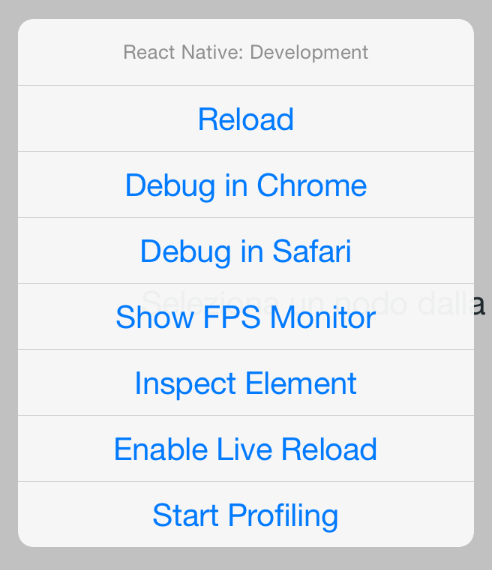
\includegraphics[width=\textwidth*1/3]{../immagini/rn-devmenu}
\caption{Developer menu di React Native}  
\end{figure}

Il menù è composto dalle voci:
\begin{itemize}
\item \textbf{Reload}: permette di ricaricare il bundle dell'applicazione.
\item \textbf{Debug in ...}: permette di eseguire il debug dell'applicazione utilizzando Chrome o Safari, maggiori informazioni sono disponibili nella sezione §\ref{sec:chrome}.
\item \textbf{Show FPS Monitor}: permette di visualizzare il numero di \gls{FPS} dell'interfaccia grafica dell'applicazione.
\item \textbf{Inspect Element}: permette di analizzare i vari componenti dell'interfaccia grafica, visualizzando, per ogni componente selezionato, i componenti che lo contengono, lo stile del componente e le dimensioni effettive del componente.
\item \textbf{Enable Live Reload}: quando abilitato l'applicazione viene ricaricata in modo automatico ad ogni modifica subita dai file sorgenti.
\item \textbf{Start Profiling}: permette di visualizzare gli stack delle chiamate durante l'esecuzione dell'applicazione, relativi sia alla parte Obj-C, sia alla parte JavaScript. 
\end{itemize}

Questo menù viene rimosso automaticamente quando l'applicazione viene compilata per essere pubblicata nello store.

\section{Flux}\label{sec:flux}
Flux è un pattern architetturale per le applicazioni sviluppate con React e React Native proposto da Facebook.

L'obiettivo di questo pattern è quello di organizzare la gestione dei dati dell'applicazione in modo che ci sia un flusso di dati unidirezionale sfruttando il sistema di composizione dei componenti di React.

Il flusso parte da degli oggetti \textit{stores}, che contengono i dati dell'applicazione, questi dati vengono poi prelevati da alcuni  componenti \textit{smart} dell'applicazione, che a loro volta li forniscono ai componenti che li compongono.

Per modificare i dati presenti in uno \textit{store} è necessario creare un oggetto \textit{action} che, mediante il \textit{dispatcher} dell'applicazione, viene ricevuto dai vari \textit{stores}, i quali lo utilizzano per aggiornare i dati che contengono.

%Quando un componente vuole modificare i dati presenti in uno \textit{store}, deve creare un oggetto \textit{action} che, mediante il \textit{dispatcher} dell'applicazione, viene ricevuto dai vari \textit{stores}, i quali lo utilizzano per aggiornare i dati che contengono.

\begin{figure}[htp]
\centering
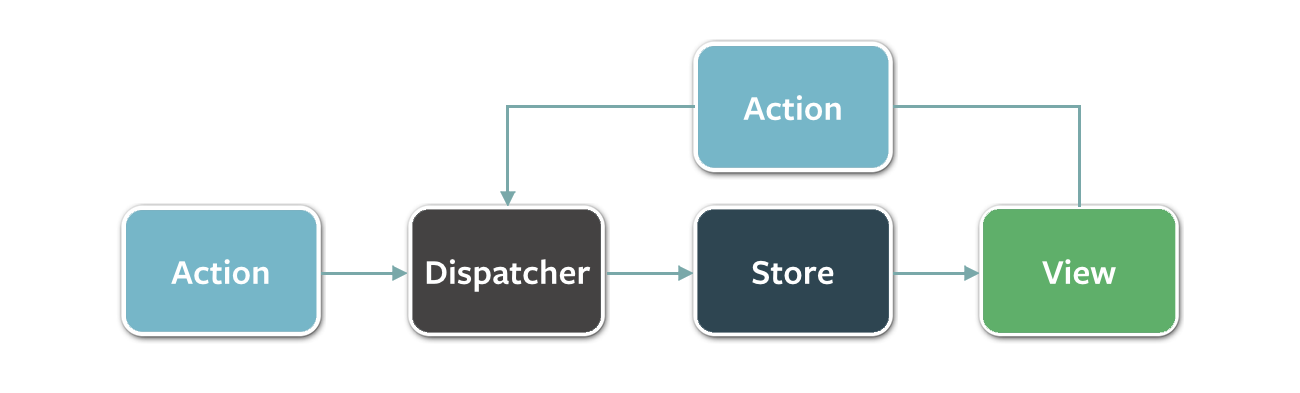
\includegraphics[width=\textwidth*3/4]{../immagini/flux-simple}
\caption{Diagramma del pattern Flux}  
\end{figure}
\FloatBarrier

Come anticipato, Flux prevede tre tipologie principali di componenti:
\begin{itemize}
\item \textbf{Stores:} sono dei \gls{singleton} che contengono i dati dell'applicazione e che forniscono solamente dei metodi \textit{getter} per recuperarli. Una volta creati, gli \textit{stores} restano in attesa dell'esecuzione di un \textit{action}, la quale può essere utilizzata per aggiornare i dati contenuti nello \textit{store}.
\item \textbf{Actions:} sono degli oggetti che contengono delle informazioni riguardante alle varie operazioni che possono eseguite dagli \textit{stores} dell'applicazione. Tipicamente vengono create dai \textit{view-controller} di React e contengono già i dati necessari agli \textit{stores} per aggiornarsi. Nel caso di operazioni asincrone i \textit{view-controller} creano l'azione che verrà comunicata al \textit{dispatcher} solamente quando le istruzioni asincrone sono state completate.
\item \textbf{Dispatcher:} oggetto che riceve un \textit{action} e ne esegue il broadcast verso tutti gli \textit{stores} dell'applicazione. Fornisce delle funzionalità che permettono ai vari \textit{stores} di registrarsi e di specificare eventuali dipendenze verso altri \textit{stores}, in modo che un determinato \textit{store} venga aggiornato una volta completato l'aggiornamento degli \textit{stores} da cui dipende, evitando così di ottenere uno stato inconsistente.


%che l'aggiornamento di un determinato \textit{store} venga effettuato solamente quando gli \textit{stores} da cui dipende abbiano finito di aggiornarsi, evitando così di ottenere uno stato inconsistente.
\end{itemize}


\subsection{Sequenza delle azioni}

\begin{figure}[htp]
\centering
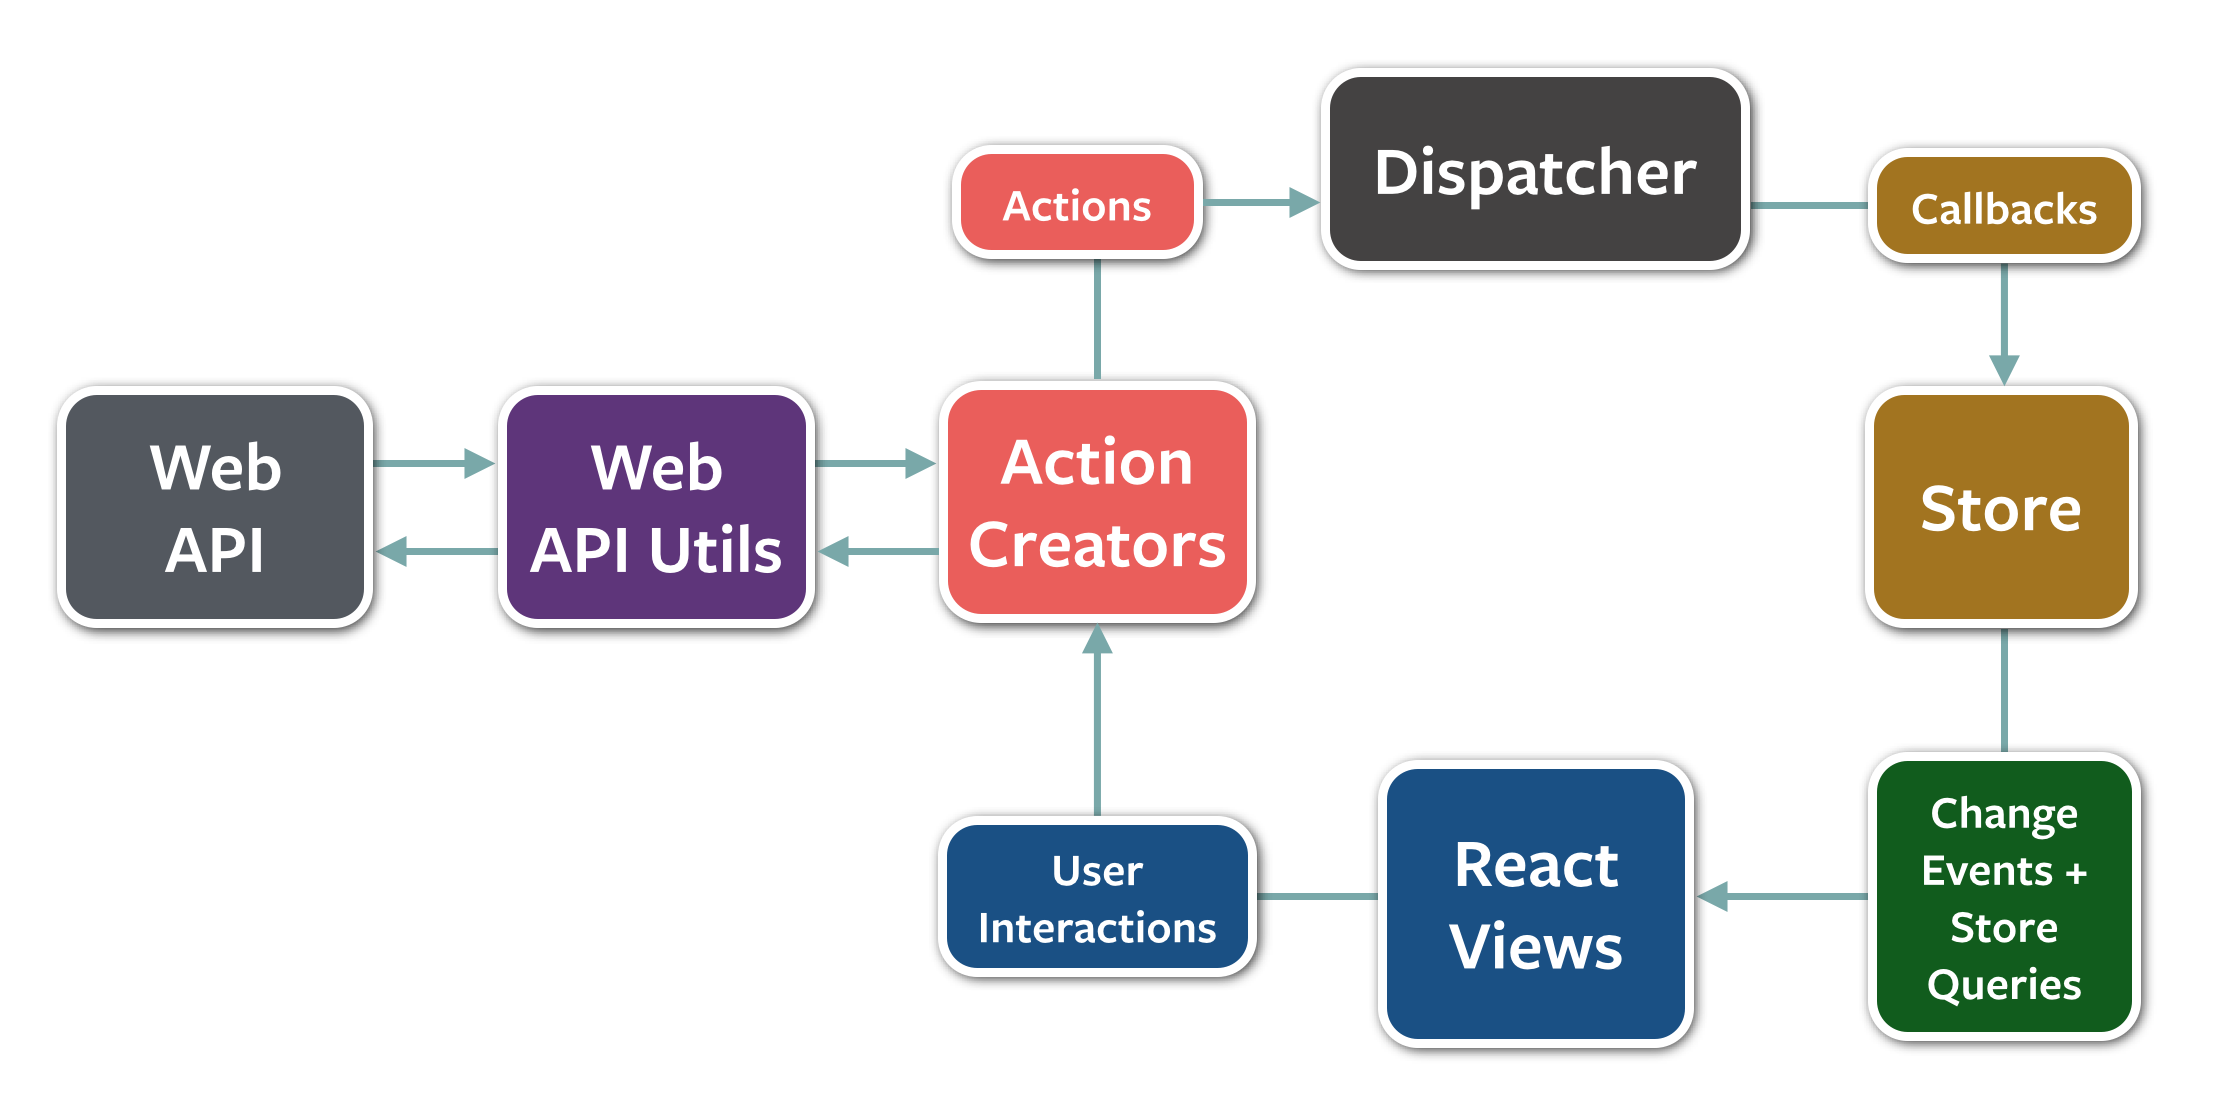
\includegraphics[width=\textwidth*3/4]{../immagini/flux-diagram}
\caption{Funzionamento del pattern Flux}  
\end{figure}
\FloatBarrier

\begin{enumerate}
\item L'utente esegue un'azione sulla view.
\item Il gestore dell'evento crea un \textit{action} e la comunica al \textit{dispatcher}.
\item Il \textit{dispatcher} manda a tutti gli \textit{stores} registrati l'oggetto \textit{action} ricevuto.
\item Ogni \textit{store} esamina l'oggetto  \textit{action} e se necessario si aggiorna. 
\item Gli \textit{stores} che hanno subito modifiche emettono un evento per comunicare ai componenti React in ascolto che si devono aggiornare.
\item I componenti React richiedono agli \textit{stores} i dati per aggiornarsi.
\end{enumerate}

\subsection{Differenze con MVC}

Nonostante Flux ed MVC possano sembrare due pattern totalmente diversi, in realtà Flux è una variante del MVC classico con delle modifiche che lo adattano al funzionamento di React e React Native.

Infatti, con MVC, i \textit{controllers} interagiscono con il \textit{model} e le \textit{view} dell'applicazione visualizzano i dati presenti nel \textit{model}.
Quando il \textit{model} viene modificato, le \textit{view} vengono notificate e recuperano i dati aggiornati dal \textit{model}.

Mentre con Flux, i \textit{view-controller} aggiornano il \textit{model}, definito dagli \textit{stores}, in un modo più strutturato utilizzando le \textit{actions} e, una volta che l'aggiornamento degli \textit{store} è completato, questi vengono notificati in modo che possano recuperare i nuovi dati, che vengo poi passati ai componenti che compongono il \textit{view-controller}.

La logica di base è quindi la stessa, l'unica differenza è come viene effettuato l'aggiornamento dei dati, che con Flux deve passare attraverso delle \textit{actions}.

Questo vincolo imposto dall'utilizzo delle \textit{actions} permette di circoscrivere la logica di aggiornamento del \textit{model} all'interno degli \textit{stores}, limitando la complessità dell'applicazione, che nel caso di grandi applicazioni può diventare ingestibile.

Un altro vantaggio che viene dall'adozione di Flux con React riguarda l'aggiornamento dell'interfaccia grafica a seguito di una modifica dei dati, in quanto sia React che Flux ragionano a stati: con React l'interfaccia grafica visualizza uno stato dell'applicazione e un cambiamento dello stato comporta il re-rendering dell'interfaccia, mentre con Flux l'insieme degli \textit{stores} rappresenta lo stato dell'applicazione e l'esecuzione di un'azione comporta il cambiamento dello stato.

Di conseguenza è possibile collegare direttamente lo stato definito dagli \textit{stores}, con lo stato dei componenti grafici, limitando il numero di operazioni intermedie.

\subsection{flux}\label{sec:flux-npm}

\texttt{flux} è un modulo pubblicato su npm da Facebook che fornisce delle classi che aiutano nell'implementazione del pattern Flux.
Tra queste classi è presente l'implementazione completa di un \textit{dispatcher} e una classe base per la creazione degli \textit{stores} che si occupa di implementare tutta la parte relativa alla registrazione e pubblicazioni degli eventi legati all'aggiornamento dei dati.


\section{Atom e Nuclide}

Trattandosi di codice JavaScript è possibile utilizzare un qualsiasi editor di testo per sviluppare l'applicazione.
Tuttavia viene consigliato l'utilizzo di Atom, un editor open source sviluppato di GitHub, che può essere personalizzato mediante dei pacchetti.

Tra i pacchetti disponibile per Atom c'è Nuclide\footnote{\url{http://nuclide.io/}} una serie di pacchetti che aggiungo alcune funzionalità di supporto allo sviluppo con React Native, come l'auto-completamento delle keyword e l'evidenziazione della sintassi JSX.

\section{Xcode}

Nonostante il codice JavaScript possa essere scritto con qualsiasi editor di testo, è necessario utilizzare Xcode\footnote{Xcode è disponibile solamente per Mac OS X, tuttavia è possibile sviluppare applicazioni con React Native su qualsiasi sistema operativo grazie ad Exponent \url{http://exponentjs.com/}. Il funzionamento di questo servizio non è stato approfondito in quanto è stato possibile utilizzare Xcode.} per compilare l'applicazione finale in modo da poterla installare sul simulatore di iOS o su un dispositivo Apple.

Xcode rende disponibili un serie di tools per lo sviluppo delle applicazioni native che possono essere riutilizzati durante lo sviluppo di un'applicazione con React Native. Ad esempio durante l'esecuzione dell'applicazione sul simulatore di iOS è possibile controllare il consumo della memoria, il traffico dati e l'utilizzo della CPU.

\begin{figure}[htp]
\centering
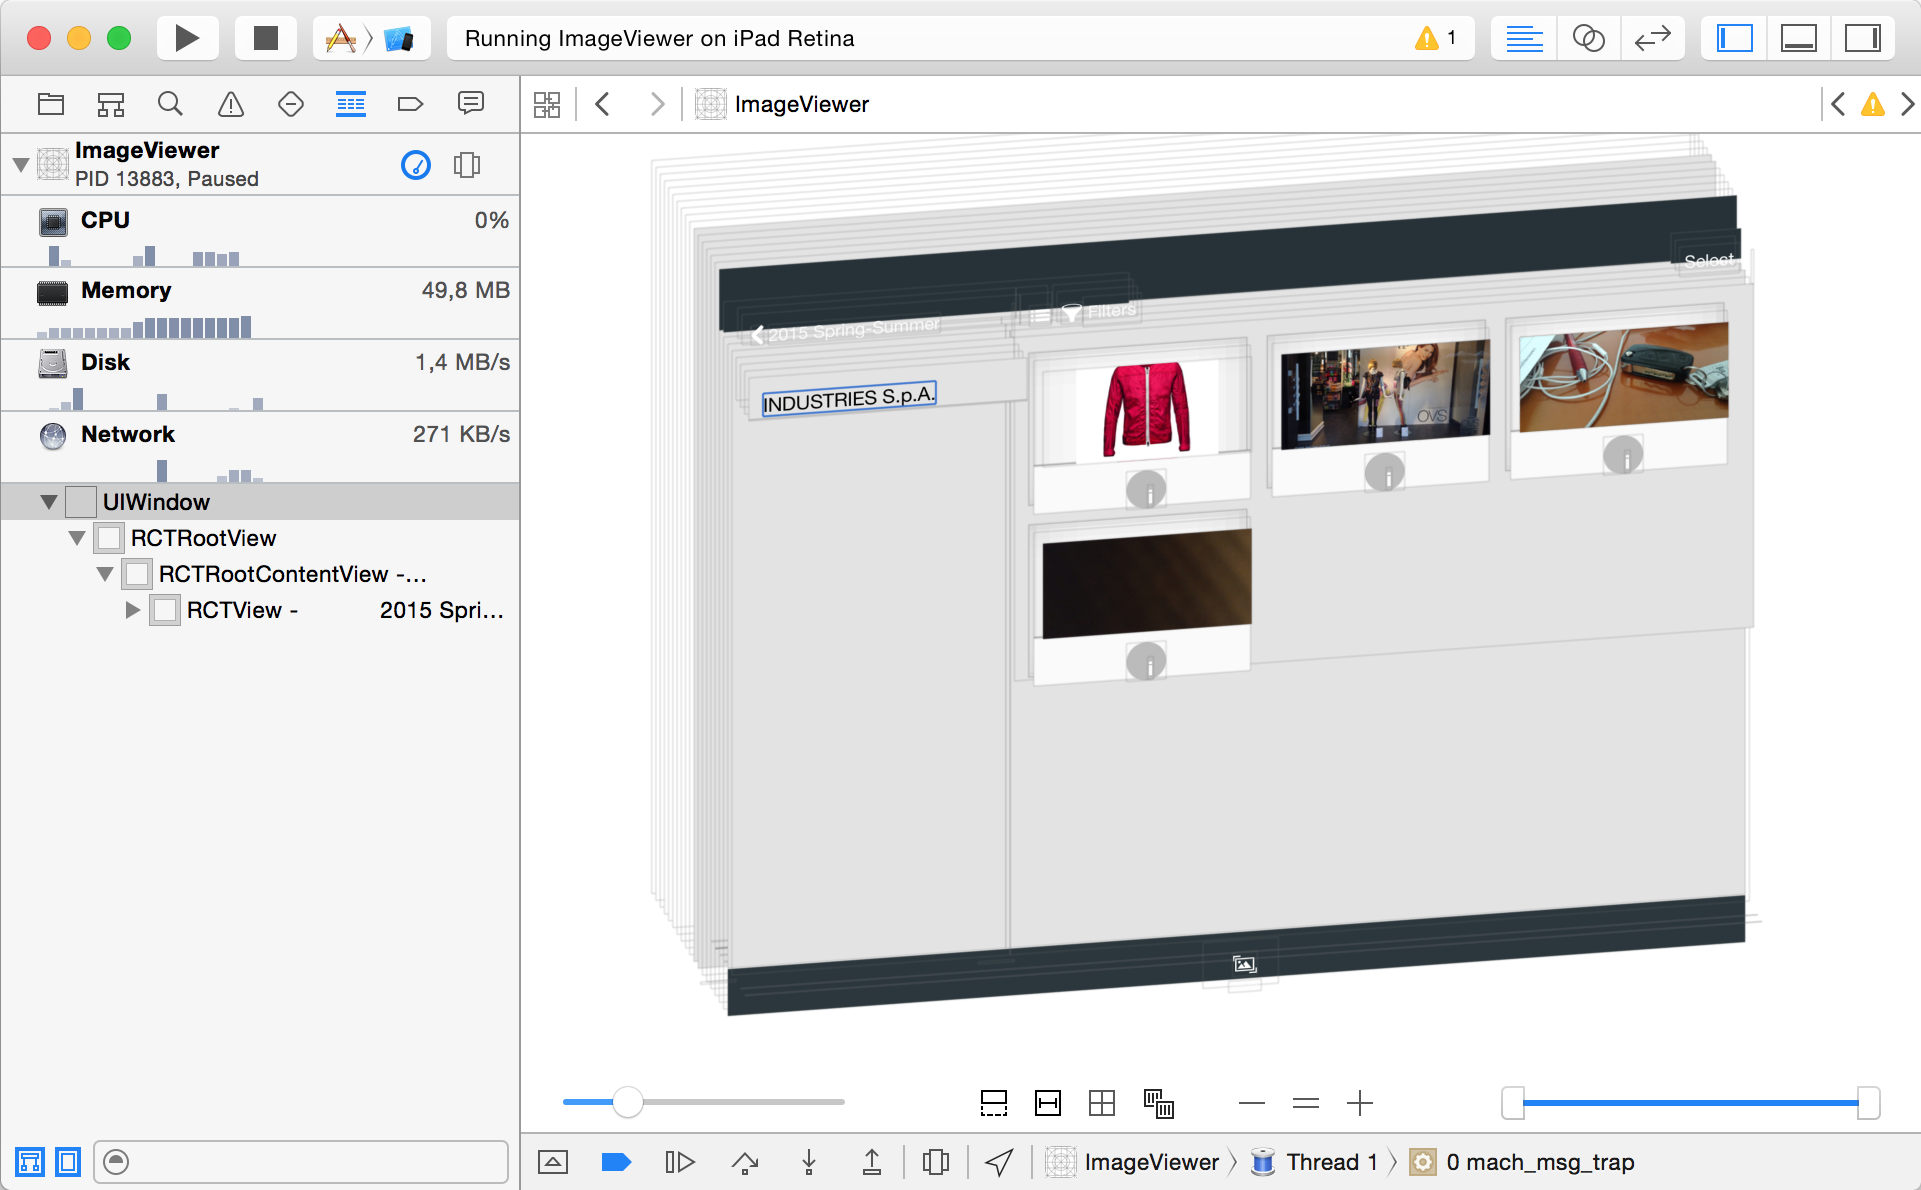
\includegraphics[width=\textwidth]{../immagini/xcode-tools}
\caption{Tools di debug di Xcode}  
\end{figure}
\FloatBarrier

\section{Google Chrome Dev Tools}\label{sec:chrome}

Durante lo sviluppo di un'applicazione con React Native è possibile utilizzare gli strumenti di sviluppo offerti da Google Chrome per effettuare il debug del codice JavaScript.

In particolare è possibile utilizzare il debugger di Chrome per inserire dei break point nel codice dell'applicazione ed effettuare l'esecuzione passo passo del codice, oppure è possibile stampare sulla console di Chrome mediante l'istruzione \texttt{console.log}.

Al momento non è possibile utilizzare tutti i tools in quanto la modalità debug di React Native utilizza una virtual machine diversa per eseguire il JavaScript.

Infatti, durante l'esecuzione normale il JavaScript viene interpretato da JavaScriptCore, mentre, durante il debug, viene utilizzata la virtual machine V8 presente all'interno di Chrome, il quale comunica con l'applicazione nativa mediante WebSocket.

In questo modo Chrome riesce a controllare l'esecuzione del JavaScript, ma non riesce ad accedere alle funzionalità che vengono eseguite dai componenti nativi, come l'utilizzo delle risorse di rete o la gestione della memoria.

\begin{figure}[htp]
\centering
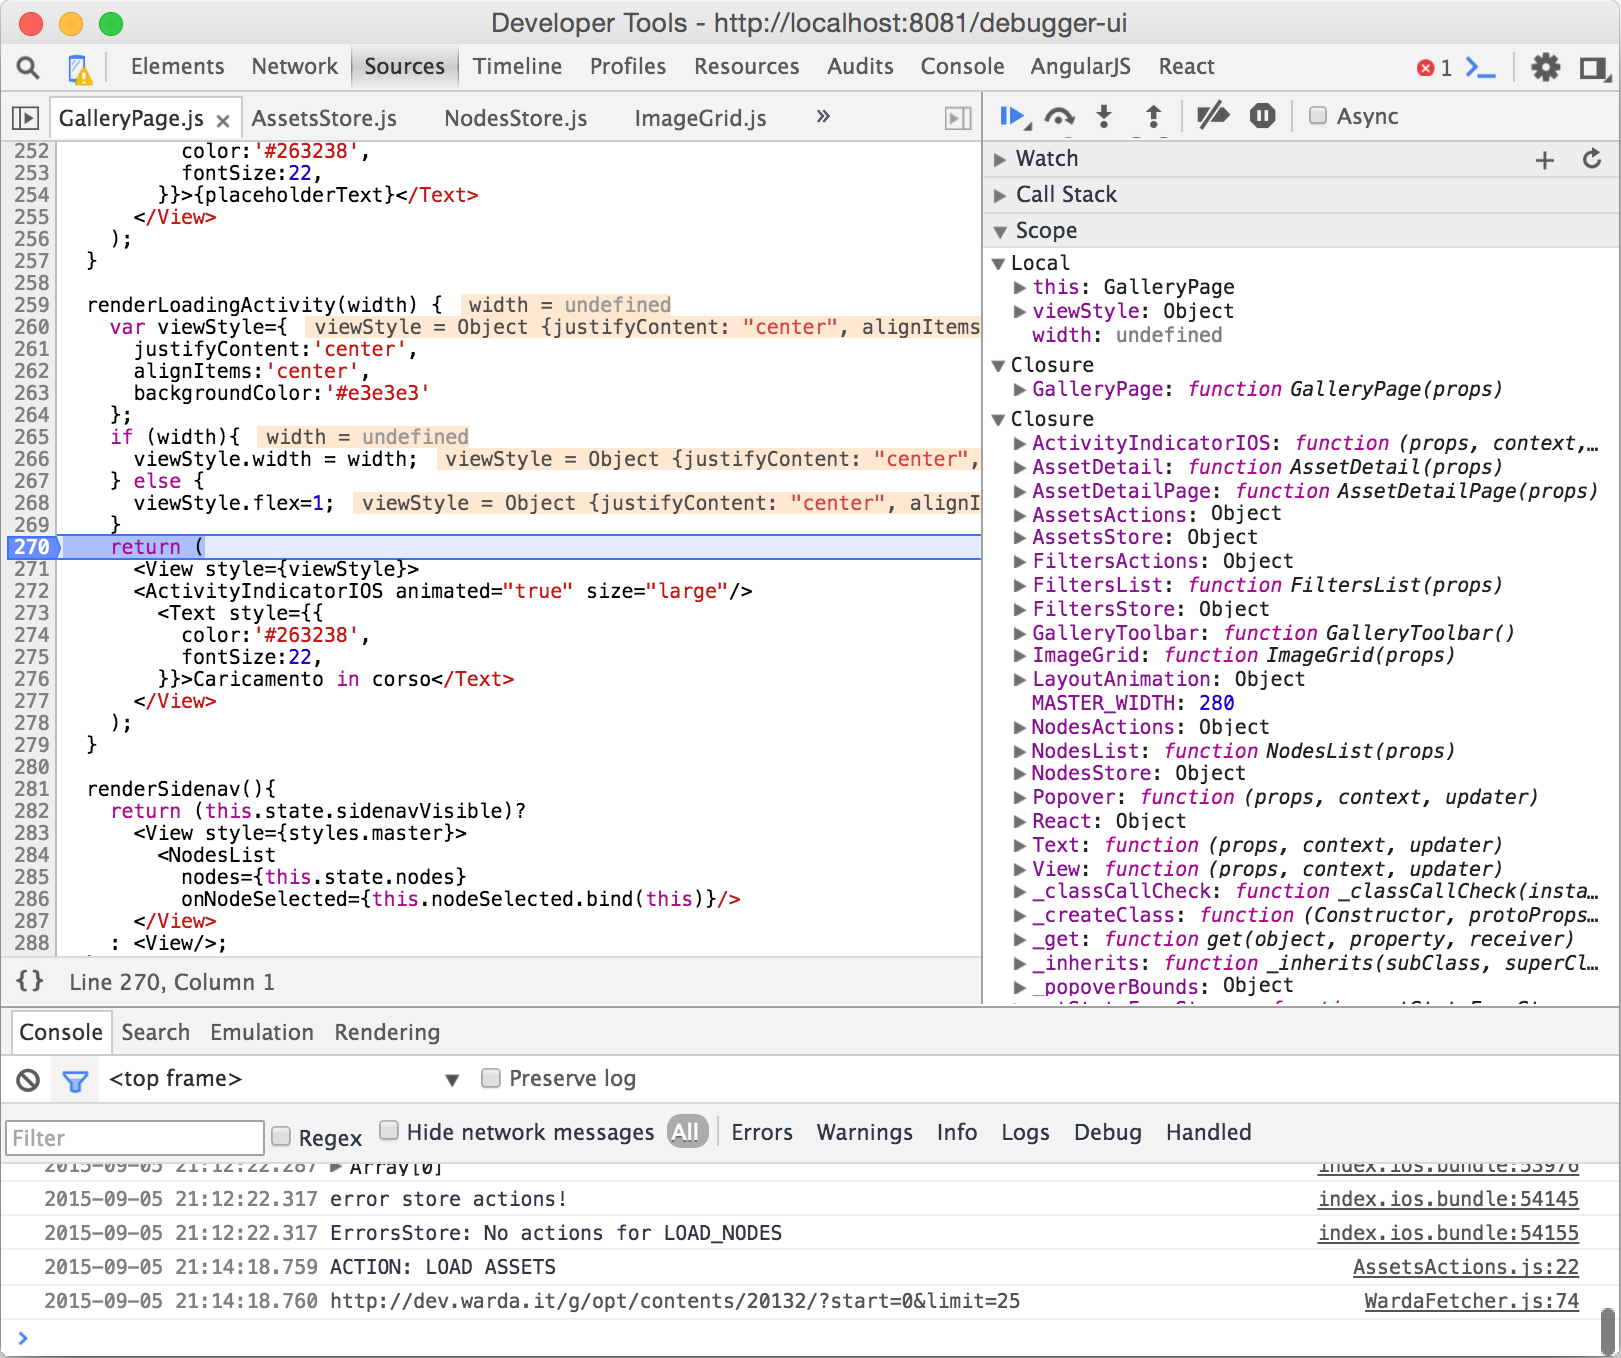
\includegraphics[width=\textwidth]{../immagini/chrome-tools}
\caption{Debug di un'applicazione con Google Chrome}  
\end{figure}

Per avviare il debug è sufficiente preme \texttt{Cmd}+\texttt{D} e selezionare l'opzione \textit{Debug in Chrome}









             
% !TEX encoding = UTF-8
% !TEX TS-program = pdflatex
% !TEX root = ../tesi.tex
% !TEX spellcheck = it-IT

%**************************************************************
\chapter{Analisi dei Requisiti}
\label{cap:analisi-dei-requisiti}
%**************************************************************

Questo capitolo contiene i requisiti dell'applicazione che sono stati individuati sia discutendo con il tutor aziendale, sia analizzando l'attuale client per iPad di WARDA.

Dal momento che lo scopo dello stage è quello di riprodurre l'applicazione attuale non è stato necessario effettuare un'analisi dei requisiti a partire dai casi d'uso, in quanto i requisiti possono essere estrapolati direttamente dall'applicazione attuale.

Il capitolo inizia quindi con la descrizione delle caratteristiche d'interesse dell'applicazione attuale per poi elencare i requisiti individuati.

%Il contenuto di questo capitolo è il risultato dei vari sprint effettuati, in quanto l'intero processo di sviluppo del prodotto è stato svolto in modo simile a quanto previsto dalla metodologia agile Scrum.

%Dopo un'analisi iniziale dell'applicazione attuale, effettuata in modo da identificare il dominio applicativo, tutte le attività sono state svolte secondo degli \textit{sprint}, ognuno dei quali mirato ad implementare una determinata caratteristica dell'applicazione.

%Ogni \textit{sprint} è stato caratterizzato da un breve riunione con il tutor aziendale, seguita da un'analisi dei nuovi requisiti emersi, per poi passare alla progettazione e all'implementazione delle nuove funzionalità.


\section{Applicazione attuale}

L'applicazione attuale per iPad di WARDA permette di visualizzare il contenuto di una gallery che si trovata sul server principale dell'applicazione.

Oltre alla visualizzazione della gallery è possibile anche creare nuovi asset, recuperando un'immagine dalla libreria interna del dispositivo o dalla fotocamera e accedere alla funzionalità collaborative offerte dalla piattaforma WARDA.

Per il progetto dello stage, l'azienda è interessata solamente alla componente gallery dell'applicazione, in quanto si tratta della parte della applicazione che richiede la maggior quantità di risorse e che attualmente soffre di alcuni problemi prestazionali.

La struttura dati alla base di una gallery realizzata con WARDA è un albero, composto da vari nodi, ognuno dei quali contiene un'insieme di assets e dei possibili filtri.

Per WARDA un'asset è un'immagine a cui vengono associati dei metadati che la descrivono, questi metadati possono poi essere utilizzati per filtrare gli assets presenti in un nodo, in modo da permettere all'utente di visualizzare solamente gli assets con determinate caratteristiche.

\subsection{Pagina di visualizzazione della gallery}

La pagina dell'applicazione che visualizza la gallery è composta da tre parti principali:
\begin{itemize}
\item una lista che visualizza i nodi figli del nodo corrente;
\item una griglia che visualizza gli asset presenti nel nodo corrente;
\item una lista di filtri che visualizza i filtri che possono essere applicati sugli assets contenuti nel nodo corrente.
\end{itemize}
Ognuno di questi componenti sarà descritto nelle seguenti sotto sezioni.

\begin{figure}[htbp]
\centering
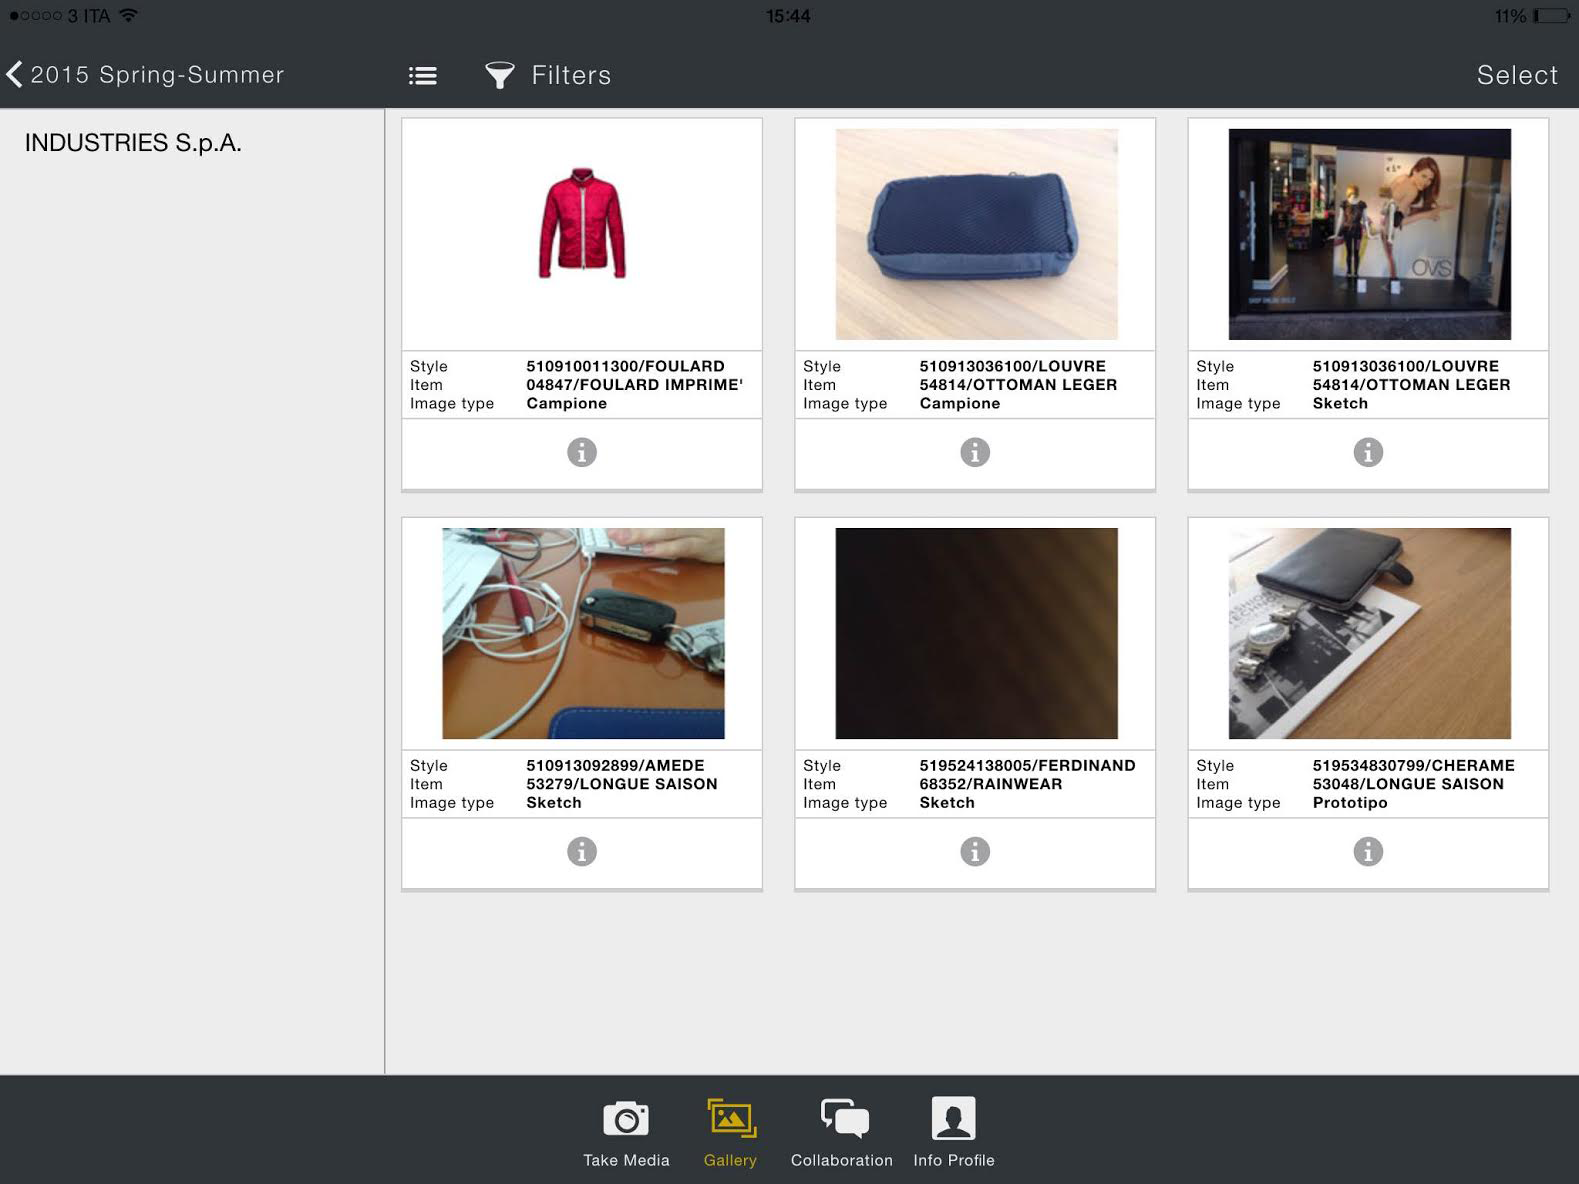
\includegraphics[width=\textwidth]{../immagini/warda-gallery}
\caption{Screenshot della gallery dell'applicazione attuale}  
\end{figure}

\subsubsection{Lista dei nodi}

\begin{figure}[htbp]
\centering
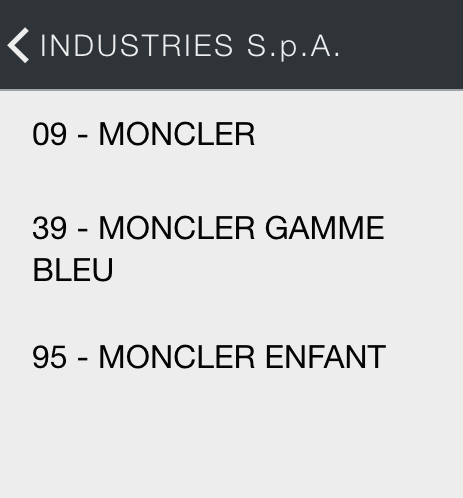
\includegraphics[scale=0.3]{../immagini/warda-gallery-lista-nodi}
\caption{Screenshot della lista dei nodi dell'applicazione attuale}  
\end{figure}

La lista dei figli del nodo corrente visualizza il titolo di ogni nodo e, quando l'utente seleziona un nodo dalla lista, questa viene aggiornata in modo che visualizzi i nodi figli del nodo selezionato. 
La selezione di un nodo dalla lista comporta anche l'aggiornamento della griglia degli assets, la quale andrà a visualizzare gli assets contenuti nel nodo selezionato.

Durante il caricamento dei dati della lista viene visualizzato un indicatore di attività per fornire all'utente un feedback riguardo l'operazione di caricamento dei dati in corso.

Sopra la lista dei nodi è presente un pulsante che permette di tornare al nodo padre del nodo correntemente visualizzato.

Questo pulsante è caratterizzato da una freccia verso sinistra e dal titolo del nodo correntemente visualizzato, nel caso il nodo corrente sia il nodo radice della gallery, il pulsante non deve essere visibile.

\FloatBarrier
\subsubsection{Griglia degli assets}

\begin{figure}[htbp]
\centering
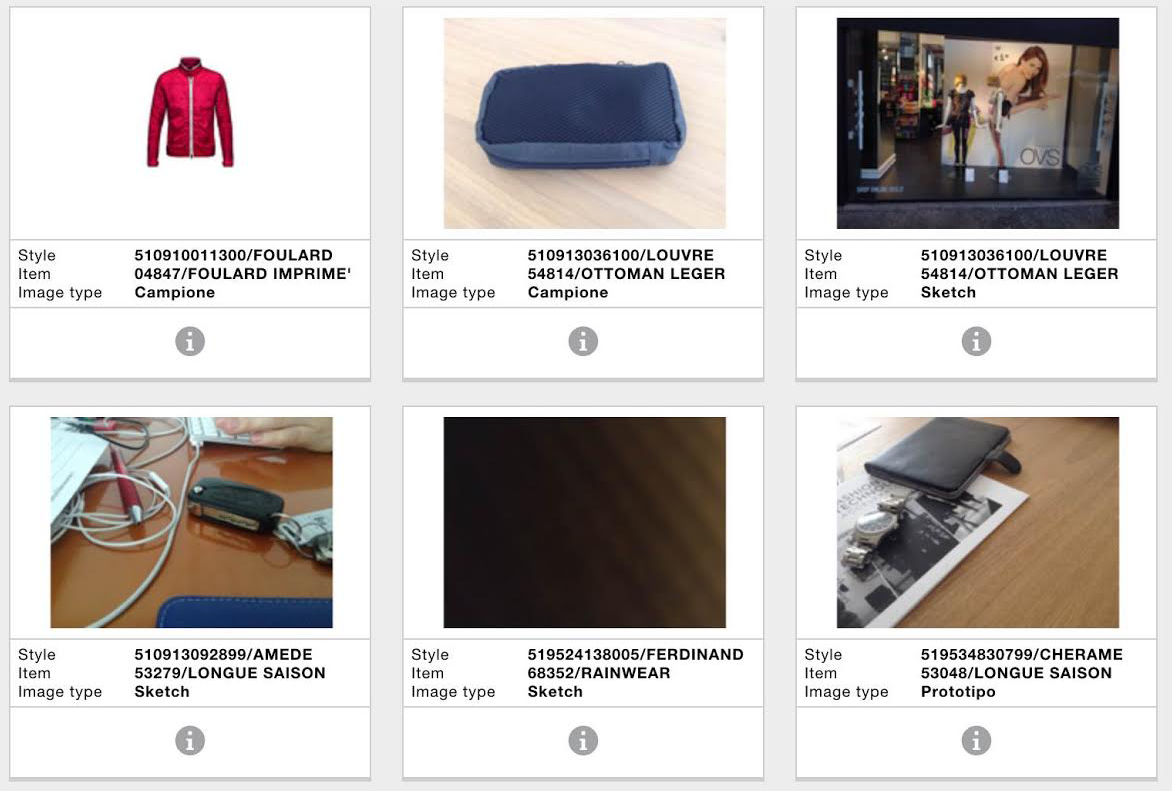
\includegraphics[width=\textwidth]{../immagini/warda-gallery-griglia}
\caption{Dettaglio della griglia degli assets dell'applicazione attuale}  
\end{figure}

La griglia degli assets rappresenta il componente principale dell'applicazione, questa griglia permette di visualizzare, per ogni asset contenuto nel nodo corrente, un'immagine di anteprima e un pulsante che permette all'utente di visualizzare i dettagli dell'asset mediante un \gls{popover}.

\begin{figure}[htbp]
\centering
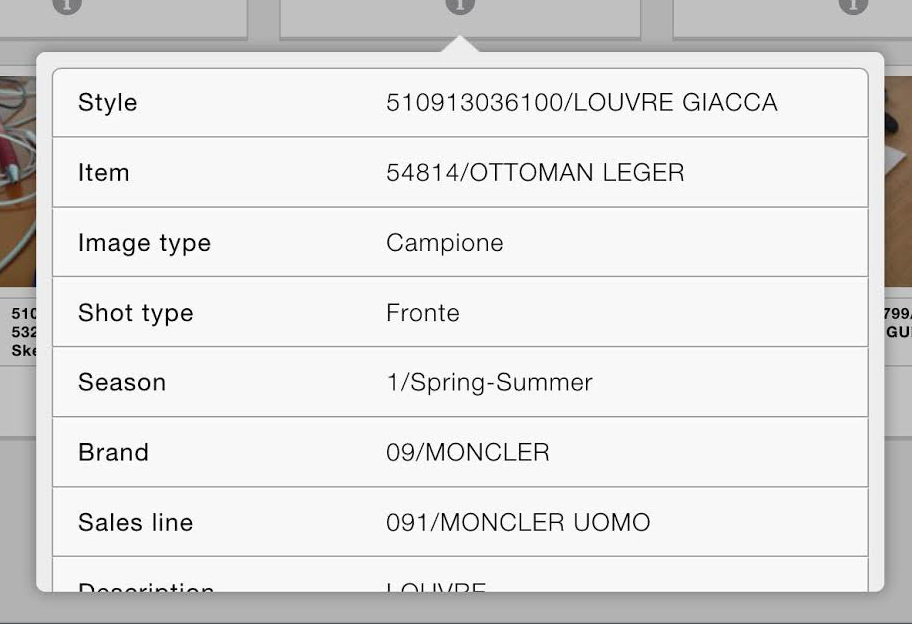
\includegraphics[scale=0.25]{../immagini/warda-gallery-dettaglio}
\caption{Popover che mostra i dettagli di un asset}  
\end{figure}

Se l'utente esegue un \gls{tap} sull'immagine di un asset, viene visualizzata una pagina dell'applicazione contenente i dettagli dell'asset e un'immagine ingrandita, maggiori informazioni riguardo questa pagina sono disponibili nella sezione §\ref{sec:pag-dettaglio-asset}.

Per motivi prestazionali, la griglia non carica subito tutti gli assets contenuti nel nodo corrente ma si limita a visualizzare solo i primi 25 assets, i successivi assets contenuti nel nodo vengono caricati man mano che l'utente prosegue nella visualizzazione della griglia, secondo il sistema dello scroll infinito.

\FloatBarrier
\subsubsection{Lista dei filtri}

\begin{figure}[htbp]
\centering
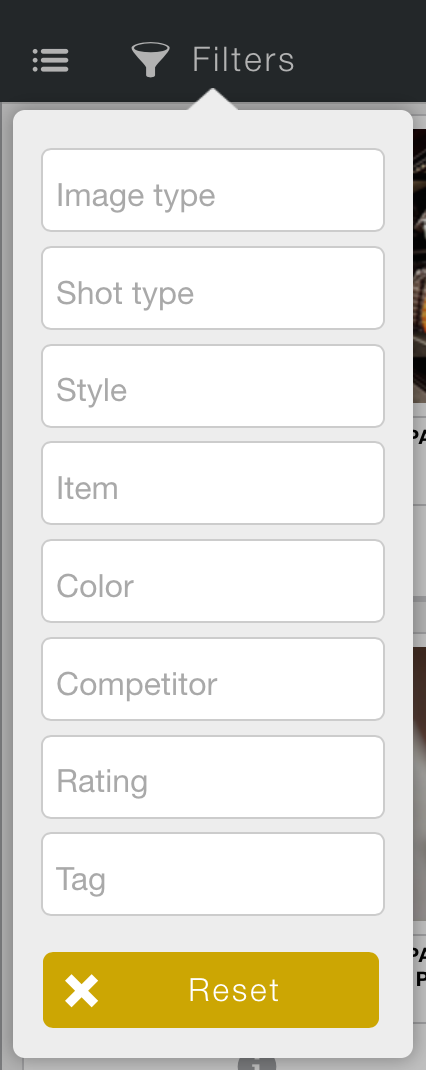
\includegraphics[scale=0.20]{../immagini/warda-filtri}
\caption{Screenshot della lista dei filtri dell'applicazione attuale}  
\end{figure}

La lista dei filtri compare come popover quando l'utente esegue un tap sul pulsante ``Filters'' presente nella barra di navigazione.

Per ogni filtro presente nel nodo corrente, viene visualizzata una lista dei possibili valori che possono essere assegnati al filtro ed una casella di testo che permette all'utente di filtrare i valori presenti nella lista.

\FloatBarrier
\subsection{Pagina di dettaglio di un asset}\label{sec:pag-dettaglio-asset}

Questa pagina contiene l'immagine ingrandita di un asset e una lista con tutti i dettagli dell'asset.

Mediante un apposito pulsante l'utente può nascondere o rendere visibile la lista dei dettagli, in modo da lasciare più spazio all'immagine.

Sull'immagine l'utente può eseguire alcune gesture:
\begin{itemize}
\item \gls{swipe} verso sinistra, per visualizzare l'asset successivo contenuto nel nodo visualizzato dalla gallery;
\item swipe verso destra, per visualizzare l'asset precedente contenuto nel nodo visualizzato dalla gallery;
\item pinch-to-zoom, per ingrandire ulteriormente l'immagine.
\end{itemize}

Infine, nella barra di navigazione della pagina è presente un pulsante che permette all'utente di tornare alla pagina con la visualizzazione a griglia.

\begin{figure}[htp]
\centering
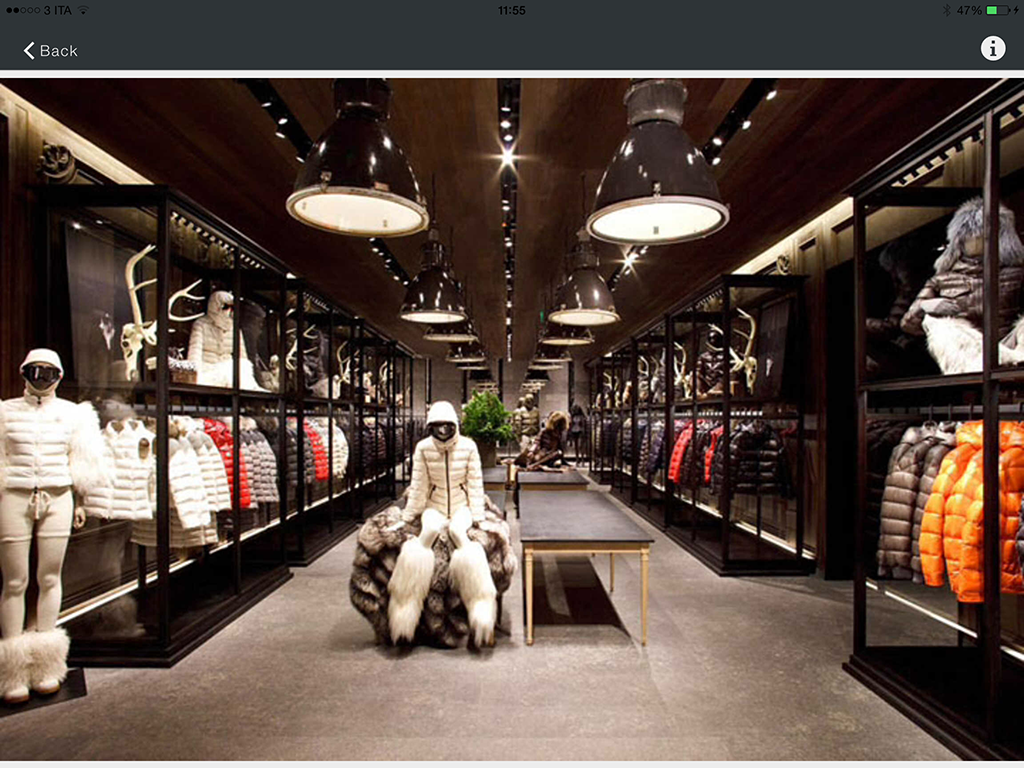
\includegraphics[scale=0.25]{../immagini/warda-asset-no-dettaglio}
\caption{Pagina di dettaglio di un asset}
\end{figure}

\begin{figure}[htp]
\centering
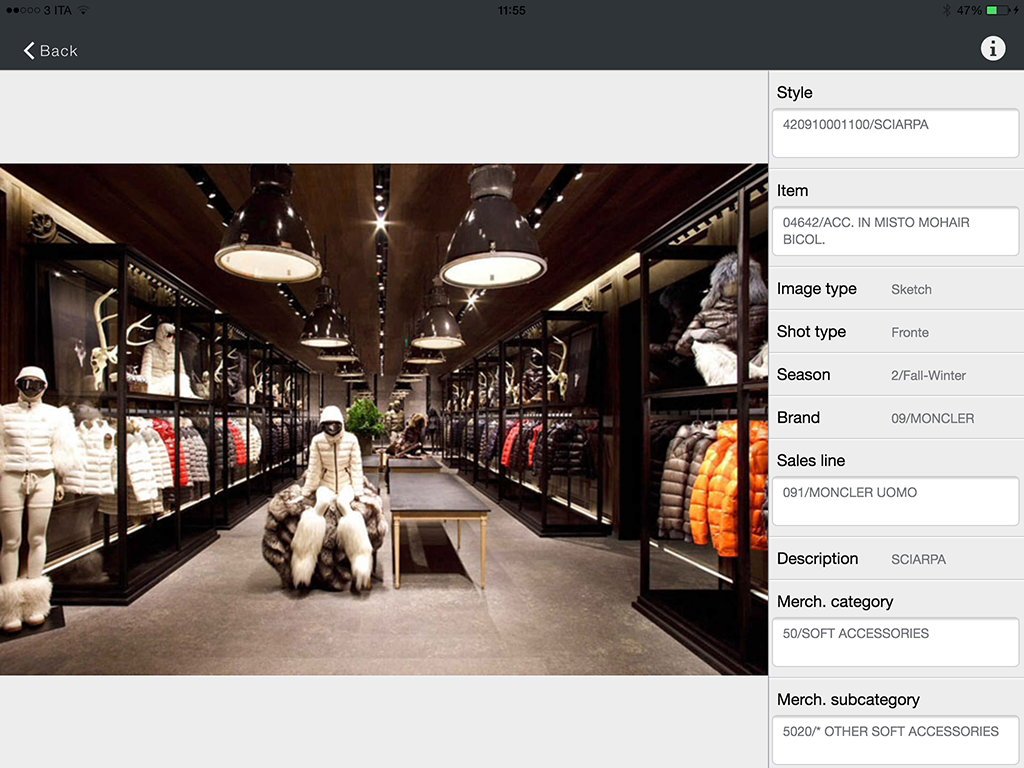
\includegraphics[scale=0.25]{../immagini/warda-asset-dettaglio}
\caption{Pagina di dettaglio di un asset con i dettagli visibili}
\end{figure}
\FloatBarrier
%
%\subsection{Utente tipo}
%L'utente tipo dell'applicazione è una persona che lavora nel mercato della moda e del lusso ed è a conoscenza del funzionamento dei processi di business legati a tale mercato.
%
%Tipicamente l'utente utilizza già il client per desktop di WARDA e vuole utilizzare l'applicazione mobile per consultare velocemente il catalogo degli assets ed eventualmente crearne di nuovi.
%
%Influenzato dall'esperienza con altre applicazioni e dal mondo in cui lavora, l'utente si aspetta che l'applicazione per iPad sia performante e che sia dotata di un interfaccia grafica accattivante e personalizzabile.

\section{Requisiti individuati}

I requisiti individuati dall'analisi dell'applicazione attuale e dalle discussioni con il tutor aziendale sono stati catalogati secondo il codice:
\begin{center}
\textit{R[T][I][C]}
\end{center}
dove:
\begin{itemize}
\item \textbf{T}ipo: specifica la tipologia del requisito e può assumere i seguenti valori:
	\begin{itemize}
	\item \textbf{F} - \textit{funzionale}, cioè che determina una funzionalità dell'applicazione;
	\item \textbf{V} - \textit{vincolo}, che riguarda un vincolo che il prodotto deve rispettare.
	\end{itemize}
\item \textbf{I}mportanza: specifica l'importanza del requisito e può assumere i seguenti valori:
	\begin{itemize}
	\item \textbf{O} - \textit{obbligatorio}, il requisito corrisponde ad un obbiettivo minimo del piano di stage e deve essere soddisfatto per garantire il funzionamento minimo dell'applicazione;
	\item \textbf{D} - \textit{desiderabile}, il requisito corrisponde ad un obbiettivo massimo del piano di stage e deve essere soddisfatto per garantire il funzionamento dell'applicazione;
	\item \textbf{F} - \textit{facoltativo}, indica che il requisito fornisce del valore aggiunto all'applicazione e non era stato previsto nel piano di stage.
	\end{itemize}
\item \textbf{C}odice: rappresenta un codice che identifica il requisito all'interno di una gerarchia. Questo codice è definito in modo che il requisito \textit{RTIx.y} sia un requisito che va a definire con un grado maggiore di dettaglio alcuni degli aspetti del requisito \textit{RTIx}.
\end{itemize}

%subsection
\subsection{Requisiti Funzionali}
\normalsize
\begin{longtable}{|c|m{10cm}|}
\hline
\textbf{Id Requisito} & \textbf{Descrizione}\\
\hline
\endhead
RFO1 & L'utente deve poter visualizzare una gallery dell'applicazione WARDA a partire dal nodo radice della gallery \\ \hline
RFO1.1 & L'utente deve poter visualizzare la lista dei nodi contenuti nel nodo correntemente visualizzato \\ \hline
RFD1.1.1 & Durante il caricamento della lista dei nodi, deve essere presente un indicatore di attività per evidenziare l'attività in corso \\ \hline
RFD1.2 & L'utente deve poter rendere visibile la lista dei nodi contenuti nel nodo corrente \\ \hline
RFF1.2.1 & La comparsa della lista dei nodi deve avvenire in modo animato \\ \hline
RFD1.3 & L'utente deve poter nascondere la lista dei nodi dei nodi contenuti nel nodo corrente \\ \hline
RFF1.3.1 & La scomparsa della lista dei nodi deve avvenire in modo animato \\ \hline
RFO1.4 & L'utente deve poter spostarsi tra i nodi presenti in una gallery \\ \hline
RFO1.4.1 & L'utente deve poter selezionare un nodo contenuto nel nodo corrente per visualizzarne i contenuti \\ \hline
RFO1.4.2 & L'utente deve poter ritornare al nodo precedente visualizzato \\ \hline
RFF1.4.3 & Il cambiamento degli elementi presente nella lista dei nodi deve essere animato \\ \hline
RFO1.4.4 & Lo spostamento da un nodo all'altro deve comportare l'aggiornamento della lista dei nodi figli e della lista degli assets \\ \hline
RFO1.5 & L'utente deve poter visualizzare la lista degli assets contenuti nel nodo correntemente visualizzato \\ \hline
RFD1.5.1 & Durante il caricamento degli elementi della lista, deve essere presente un indicatore di attività per evidenziare l'attività in corso \\ \hline
RFO1.5.2 & La lista contenente gli assets deve avere un layout a griglia \\ \hline
RFO1.5.3 & La lista deve visualizzare un numero limitato di assets ed essere dotata di un sistema di scroll infinito \\ \hline
RFO1.5.3.1 & Una volta che l'utente visualizza tutti gli assets contenuti della griglia, se presenti, devono essere caricati ulteriori assets \\ \hline
RFO1.5.3.2 & Durante il caricamento degli ulteriori assets deve essere presente un indicatore di attività \\ \hline
RFO1.5.4. & Gli elementi della lista degli assets devono essere composti da un'immagine di anteprima dell'asset e da un pulsante ``Info'' \\ \hline
RFO1.5.4.1 & Quando l'utente esegue un tap sull'immagine di anteprima di un asset, deve essere visualizzata la pagina di dettaglio dell'asset \\ \hline
RFO1.5.4.2 & Quando l'utente esegue un tap sul pulsante Info di un asset, deve essere visualizzato un popover contenente le informazioni di dettaglio dell'asset \\ \hline
RFO1.6 & L'utente deve poter visualizzare la lista dei filtri disponibili per il nodo correntemente visualizzato \\ \hline
RFO1.6.1 & Per ogni filtro disponibile, l'utente deve poter visualizzare tutti i valori che può assumere il filtro \\ \hline
RFD1.6.1.1 & L'utente deve poter cercare un determinato valore all'interno della lista dei valori che può assumere il filtro \\ \hline
RFO1.6.1.2 & L'utente deve poter selezionare un valore per il filtro da applicare \\ \hline
RFO1.6.2 & L'utente deve poter applicare più filtri contemporaneamente \\ \hline
RFO1.6.3 & L'utente deve poter rimuovre un filtro \\ \hline
RFO1.6.4 & L'utente deve poter rimuovere tutti i filtri applicati \\ \hline
RFD1.6.5 & L'utente deve poter visualizzare il numero di filtri applicati \\ \hline
RFO1.6.6 & I filitri devono rimanere attivi anche se l'utente si sposta su un altro nodo \\ \hline
RFD1.6.7 & La lista dei filtri deve essere visualizzata come un pop-up \\ \hline
RFO2 & L'utente deve poter visualizzare una pagina contenente i dettagli di un asset \\ \hline
RFO2.1 & L'utente deve poter tornare alla pagina contenente la gallery \\ \hline
RFO2.2 & L'utente deve poter visualizzare un'immagine ingrandita dell'asset \\ \hline
RFD2.2.1 & Durante il caricamento dell'immagine, deve essere presente un indicatore di attività che visualizzi la percentuale di caricamento \\ \hline
RFF2.2.2 & L'utente deve poter effettuare il pinch-to-zoom sull'immagine \\ \hline
RFO2.2.3 & L'utente deve poter effettuare uno swipe da destra verso sinistra sull'immagine, per visualizzare in dettaglio l'asset successivo secondo l'ordine del contenuto della gallery \\ \hline
RFF2.2.3.1 & Allo swipe deve essere associata un'animazione che sposti l'immagine da destra verso sinistra seguendo il movimento effettuato dall'utente \\ \hline
RFF2.2.3.2 & Nel caso non sia presente un'asset successivo da visualizzare, l'animazione dello swipe deve essere interrotta \\ \hline
RFO2.2.4 & L'utente deve poter effettuare uno swipe da sinistra verso destra sull'immagine, per visualizzare in dettaglio l'asset precedente secondo l'ordine del contenuto della gallery \\ \hline
RFF2.2.4.1 & Allo swipe deve essere associata un'animazione che sposti l'immagine da sinistra verso destro seguendo il movimento effettuato dall'utente \\ \hline
RFF2.2.4.2 & Nel caso non sia presente un'asset precedente da visualizzare, l'animazione dello swipe deve essere interrotta \\ \hline
RDO2.3 & L'utente deve poter visualizzare una lista contenente i dettagli dell'asset visualizzato \\ \hline
RFD2.4 & L'utente deve poter rendere visibile la lista contenente i dettagli dell'asset visualizzato \\ \hline
RFF2.4.1 & La comparsa della lista contenente i dettagli deve avvenire in modo animato \\ \hline
RFD2.5 & L'utente deve poter nascondere la lista contenente i dettagli dell'asset visualizzato \\ \hline
RFF2.4.1 & La scomparsa della lista contenente i dettagli deve avvenire in modo animato \\ \hline
RFF3 & L'utente deve visualizzare un messaggio d'errore nel caso l'applicazione non riesca a connettersi con il server \\ \hline
\caption[Requisiti Funzionali]{Requisiti Funzionali}
\label{tabella:req0}
\end{longtable}

\subsection{Requisiti di Vincolo}
\normalsize
\begin{longtable}{|c|m{10cm}|}
\hline
\textbf{Id Requisito} & \textbf{Descrizione} \\
\hline
\endhead
RVD1 & L'applicazione deve essere dotata di un file di configurazione che permette di impostare: l'indirizzo del server a cui connettersi, l'id della gallery da visualizzare, l'username e password con i dati da utilizzare per effettuare l'accesso e il numero di assets da visualizzare in una singola pagina \\ \hline
RVO2 & L'applicazione deve essere realizzata con React Native \\ \hline
RVO3 & L'applicazione deve essere compatibile con iPad di seconda generazione \\ \hline
RVD4 & L'interfaccia grafica dell'applicazione deve essere fluida e non bloccarsi \\ \hline
\caption[Requisiti di Vincolo]{Requisiti di Vincolo}
\label{tabella:req1}
\end{longtable}



\section{Riepilogo requisiti}

In totale sono stati individuati 52 requisiti, ripartiti tra le varie tipologie secondo quanto riportato nelle seguenti tabelle.
\\ \\ \\
\begin{minipage}{\textwidth}
  \begin{minipage}[b]{0.49\textwidth}
    \centering
      \begin{tabular}{|l|c|} \hline
      \textbf{Importanza} & \textbf{\#} \\ \hline
  Obbligatori & 29 \\ \hline
  Desiderabili & 12 \\ \hline
  Facoltativi & 11 \\ \hline
  Totale & 52 \\ \hline
\end{tabular}
      \captionof{table}{Numero di requisiti per importanza}
	\end{minipage}
	  \hfill
  \begin{minipage}[b]{0.49\textwidth}
    \centering
         \begin{tabular}{|l|c|} \hline
      \textbf{Tipologia} & \textbf{\#} \\ \hline
  Funzionali & 48 \\ \hline
  Vincolo & 4 \\ \hline
    Totale & 52 \\ \hline
\end{tabular}
    \captionof{table}{Numero di requisiti per tipologia}
  \end{minipage}
\end{minipage}
 \\ \\ \\

\begin{minipage}{\textwidth}
  \begin{minipage}[b]{0.49\textwidth}
    \centering
    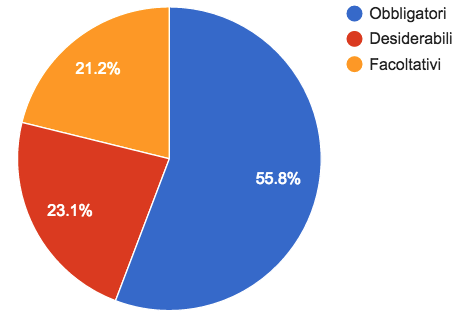
\includegraphics[scale=0.7]{../immagini/requisiti-totale-importanza}
      \captionof{figure}{Requisiti per importanza}
	\end{minipage}
	  \hfill
  \begin{minipage}[b]{0.49\textwidth}
    \centering
  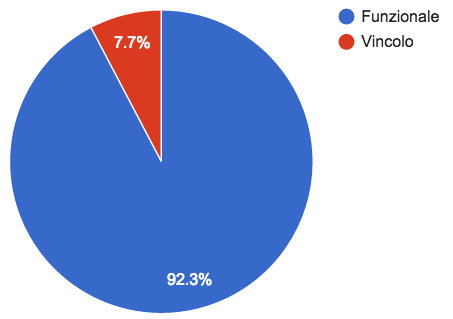
\includegraphics[scale=0.7]{../immagini/requisiti-totale-tipologia}
      \captionof{figure}{Requisiti per tipologia}
  \end{minipage}
\end{minipage}



             

\appendix                               

\chapter{Gitflow}

Gitflow è un modello di sviluppo basato su Git, ideato da Vincent Driessen e presentato nel 2010 in un suo celebre post.\footnote{\url{http://nvie.com/posts/a-successful-git-branching-model/}}. Sebbene sia pittosto complicato rispetto ad altri modelli, questo framework fornisce un robusto strumento per la gestione di progetti di grandi dimensioni.

Gitflow assegna ruoli specifici ai diversi branch, specificando quando e come essi debbano interagire tra di loro. Essendo basato su Git gli sviluppatori lavorano in locale e periodicamente effettuano \textit{push} sul repository remoto centrale.

\section{I branch principali}

Nel repository principale si distinguono due rami principali:

\begin{itemize}

\item \textbf{master}, il ramo principale all'interno del quale risiede codice verificato e pronto per essere spedito in \textit{production} e in particolare tutti i suoi nodi corrispondono a \textbf{release} del prodotto, ovvero ad una versione stabile, che può essere marcata o meno con un \textit{tag};

\item \textbf{develop}, il ramo all'interno del quale avviene lo sviluppo vero e proprio del prodotto e dal quale il codice può essere rilasciato, effettuando dunque un \textit{merge} con il ramo master

\end{itemize}

\section{I branch di supporto}

Al livello inferiore dei branch principali troviamo i branch di supporto, che assistono gli sviluppatori nelle operazioni quotidiane di sviluppo. Questi branch, a differenza dei due principali, hanno un tempo di vita limitato e vengono uniti nei rami principali o semplicemente scartati. I tre branch di supporto sono:

\begin{itemize}

\item \textbf{Feature}, che viene creato dal ramo \texttt{develop} ed unito solamente nel medesimo; la loro utilità, come dice la parola stessa, è quella di creare un ramo di sviluppo per un nuovo componente del sistema. Essi normalmente vanno tenuti in locale e non devono essere \textit{pushati} sul repository remoto;

\item \textbf{Release}, che viene creato dal ramo \texttt{develop} ed unito sia nel medesimo che successivamente su \texttt{master}. Questo branch identifica le procedure che vengono istanziate all'atto della release. Quando uno sviluppatore decide di effettuare una release del prodotto apre innanzitutto un brach da \texttt{develop} chiamato \texttt{release-*}, esegue tutte le operazioni di \textit{pre-release}, effettua il merge su \texttt{develop} ed infine il merge su \texttt{master}, marcando il nodo di merge eventualmente con un \textit{tag};

\item \textbf{Hotfix}, che viene creato dal ramo \texttt{master} ed unito prima sia nel medesimo che successivamente su \texttt{develop}. Questi rami derivano dall'immediata necessità di risolvere un \textit{bug} inserito all'interno del ramo master, senza dover effettuare una nuova release. 

\end{itemize}

\begin{figure}[htp]
\centering
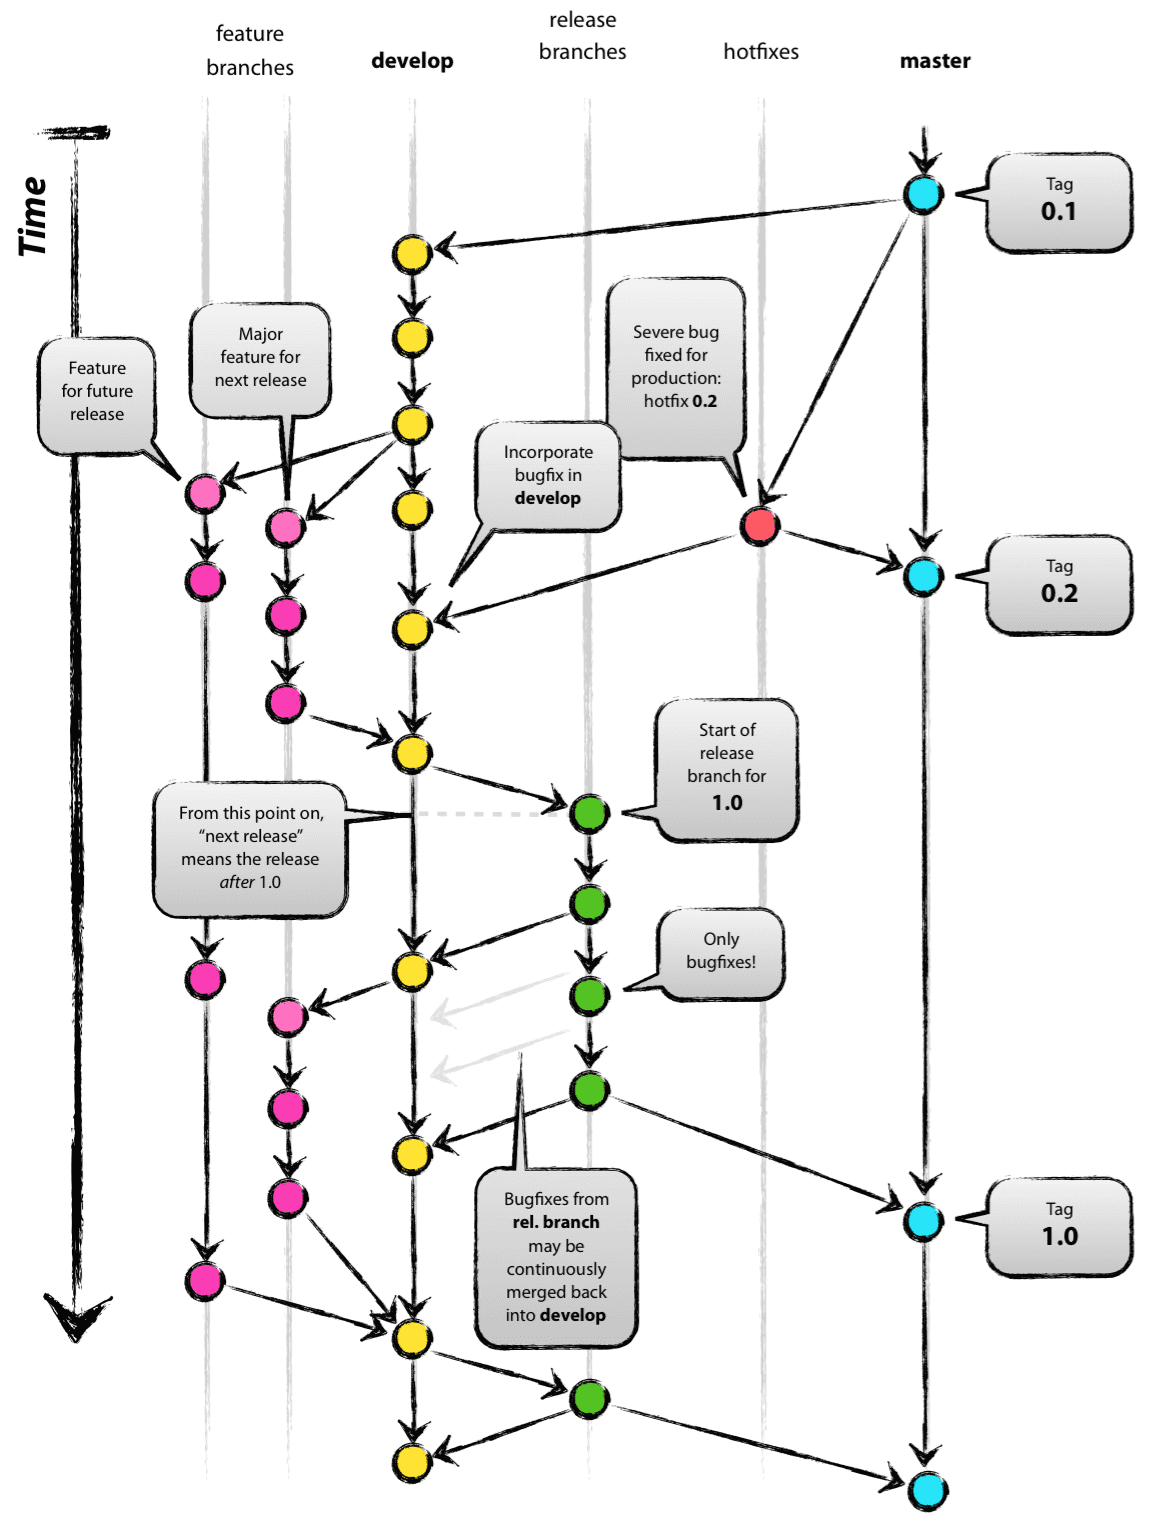
\includegraphics[width=\textwidth/2]{../immagini/git-flow-model}
\caption{Modello Gitflow}
\end{figure}


             % Appendice A

%**************************************************************
% Materiale finale
%**************************************************************
\backmatter
\printglossaries
% !TEX encoding = UTF-8
% !TEX TS-program = pdflatex
% !TEX root = ../tesi.tex
% !TEX spellcheck = it-IT

%**************************************************************
% Bibliografia
%**************************************************************

\nocite{*}
\printbibliography

\bibbycategory % equivale a dare un \printbibliography per ogni categoria


\end{document}